%        File: thesis.tex
%     Created: Tue Feb 16 06:00 PM 2016 J
% Last Change: Tue Feb 16 06:00 PM 2016 J
%
\input{../dummy/dummy.tex}
\documentclass[submit]{ipsj_v2/UTF8/ipsj}
%\documentclass{ipsj}

\usepackage{latexsym}
\usepackage[dvipdfmx]{graphicx}
\usepackage{amssymb}
\usepackage{enumerate,cite,url}
\usepackage{listings,jlisting}
\lstset{%
    language={c},%
    basicstyle={\small},%
    identifierstyle={\small},%
    commentstyle={\small\itshape},%
    keywordstyle={\small},%\bfseries},%
    ndkeywordstyle={\small},%
    stringstyle={\small\it},
    frame={tb},
    breaklines=true,
    columns=[l]{fullflexible},%
    numbers=left,%
    xrightmargin=0zw,%
    xleftmargin=3zw,%
    numberstyle={\scriptsize},%
    stepnumber=1,
    numbersep=1zw,%
    %lineskip=-0.5ex%
}

\def\Underline{\setbox0\hbox\bgroup\let\\\endUnderline}
\def\endUnderline{\vphantom{y}\egroup\smash{\underline{\box0}}\\}
\def\|{\verb|}

\setcounter{巻数}{57}
\setcounter{号数}{1}
\setcounter{page}{1}


\受付{2015}{3}{4}
%\再受付{2015}{7}{16}   %省略可能
%\再再受付{2015}{7}{20} %省略可能
\採録{2015}{8}{1}




\begin{document}


\title{Bluetoothを用いたマルチVM対応\\mrubyバイトコードローダ}

\etitle{mruby Bytecode Loader Using Bluetooth in Multi-VM Environment}

\affiliate{IPSJ}{情報処理学会\\
IPSJ, Chiyoda, Tokyo 101--0062, Japan}


\paffiliate{JU}{情報処理大学\\
Johoshori University}

\author{山本 拓朗}{Takuro Yamamoto}{IPSJ}[joho.taro@ipsj.or.jp]
\author{大山 博司}{Hiroshi Oyama}{IPSJ}
\author{安積 卓也}{Takuya Azumi}{IPSJ,JU}[gakkai.jiro@ipsj.or.jp]

\begin{abstract}
近年,組込みシステムは複雑化・大規模化しているため,組込みソフトウェアの生産性が問題になっている.

組込みソフトウェア開発の生産性の向上を目的として,mruby(軽量Ruby)を適用させたコンポーネントベース開発が可能なフレームワークであるmruby on TECSを提案してきた.

現状のmruby on TECSでは,プラットフォームにmrubyバイトコードを組み込んでいるため,mrubyプログラムを修正する度にコンパイル・リンクし直す必要がある.
さらに,マルチVMを提供しているが,複数のmrubyプログラムを効率よく並行動作させるには開発者がリアルタイムOSの機能を熟知している必要がある.

本研究では,mruby on TECSの拡張として,mrubyアプリケーションのバイトコードをBluetoothで転送することで開発効率を向上させる.
さらに,複数のmrubyプログラムを協調動作できるフレームワークを提案する.

\end{abstract}


\begin{jkeyword}
情報処理学会論文誌ジャーナル,\LaTeX,スタイルファイル,べからず集
\end{jkeyword}

\begin{eabstract}
This document is a guide to prepare a draft for submitting to IPSJ
Journal, and the final camera-ready manuscript of a paper to appear in
IPSJ Journal, using {\LaTeX} and special style files.  Since this
document itself is produced with the style files, it will help you to
refer its source file which is distributed with the style files.
\end{eabstract}

\begin{ekeyword}
IPSJ Journal, \LaTeX, style files, ``Dos and Don'ts'' list
\end{ekeyword}

\maketitle

\section{はじめに}
近年,組込みシステムは高品質・高性能化に伴い,複雑化・大規模化している.
例えば,IoTアプリケーションがある.
その上,製品の低コスト化や短期間での開発も要求されている.

ソフトウェアを効率的に開発するアプローチのひとつに,コンポーネントベース開発がある.
コンポーネントベース開発は,再利用可能なコンポーネントを構成するための設計手法である\cite{par:Crnkovic}.
コンポーネント化されたソフトウェアは,再利用性が高く,検証が容易になるため,コンポーネントベース開発を適用することで,複雑かつ大規模なソフトウェアを効率的に開発することができる.
システムの拡張や仕様変更にも柔軟に対応できる.
組込みシステムのコンポーネント技術として,TECS\cite{par:TECS}やAUTOSAR\cite{url:AUTOSAR},SaveCCM\cite{par:SAVEapproach}がある.

効率的なソフトウェア開発のもう一つのアプローチとして,スクリプト言語がある.
現在のソフトウェアのほとんどはC言語で開発されているが,C言語による開発はコストが高く,開発期間も長くなる.
スクリプト言語は,その使いやすさから高い生産性をもっているため,効率的かつ短期間での開発ができる.
有名なスクリプト言語として,Java script,Perl,Python,Lua,Rubyなどがある.

しかし,スクリプト言語は可読性や使いやすさが高い反面,C言語よりも実行時間が遅い.
組込みシステムにとって,最悪実行時間や応答時間といったリアルタイム性は非常に重要であるため,スクリプト言語を組込みシステムに利用することは難しい.

%mruby on TECSは,スクリプト言語であるmruby使用したコンポーネントベース開発が可能なフレームワークである\cite{par:mrubyonTECS}.
mruby on TECS は,mruby(軽量Ruby) と,組込みシステムに適したコンポーネントシステムであるTECS (TOPPERS Embedded Component System) を組み合わせたフレームワークである\cite{par:mrubyonTECS}.
mruby on TECS では,mruby プログラムからC 言語の関数を呼ぶ機能を提供しており,mruby に比べて,アプリケーションを約100 倍速く実行できる.

現状のmruby on TECSでは,いくつかの問題がある.
mruby on TECS は,mrubyプログラムをロードするための方法として,記憶装置しか対応していないため,作業効率が悪い.
(LEGO MINDSTORMS EV3 のプラットフォーム\cite{par:EV3})
mrubyプログラムを修正する度に,SDカードの抜き差しやROMへの書き込みを行う必要がある.
%mruby on TECS では,mruby プログラムを修正する度にターゲットデバイスでSD カードまたはROMに書き込みし,OS を再起動する必要がある.
さらに,mruby on TECS はマルチVMに対応してるが,複数のmruby アプリケーションを並行実行させる場合,開発者がタスクを待ち状態へ遷移させるOS の機能を呼び出さなければならない.

% mrubyバイトコードローダによって,開発者ははじめの一度だけ記憶装置にプラットフォーム部分を書き込み,mrubyアプリケーションのバイトコードをホストからターゲットデバイスへBluetoothを用いて転送し,実行することが可能になる.
% 繰り返してSDカードの抜き差しやROMへの書き込みをする手間が省けるため,作業効率は向上する.
% RiteVMスケジューラは複数のmrubyアプリケーションを
提案フレームワークは,mruby on TECS を拡張して,Bluetooth を用いたmruby バイトコードローダと,実用的なマルチタスク処理の実装を行った.
提案フレームワークでは,プラットフォーム部分をコンパイル・リンクし,ターゲットデバイス上で起動する.
ホストPC 側では,mruby アプリケーション(.rb) をバイトコード(.mrb) にコンパイルし,Bluetooth を通してターゲットデバイスにバイトコードを転送する. 
ターゲットデバイス側では,RiteVM に実装されたローダが転送されたバイトコードを受信し,すでにプラットフォームに含まれているmruby ライブラリと合わせてアプリケーションを実行する.
これによって,繰り返しSDカードの抜き差しやROMへの書き込みをする手間やOSを再起動する時間が省けるため,作業効率を上げることができる.
さらに,各VM の処理を平等に実行するRiteVM スケジューラを提供することで,マルチタスク処理を効率的に利用できる.

% Contribution: The proposed framework gives the contribution in the following points.
% 1) To improve the software development efficiency:
% Developers do not need to rewrite a storage/ROM device and also to restart an OS. 
% The loader supports the countinuous loading, which saves the Bluetooth setup time. 
% Therefore, the mruby bytecode loader using Bluetooth helps developers develop software.
% 2) To effectively execute multiple mruby programs in concurrent or/and parallel: 
% Developers can execute multiple tasks without the knowledge of an RTOS because the RiteVM sceduler switches tasks cyclically.
% In additon, synchronization of multiple tasks is also implemented.
% 3) To focus on the benefits of component-based developments:
% This paper shows the specific examples for the benefits of component-based development.

% Organization: The paper is organized as follows. 
% Section 2 introduces the basic technologies i.e. mruby, TECS and mruby on TECS. 
% Section 3 describes the design and implementation of the proposed framework in detail. 
% Section 4 evaluates the proposed framework, Section 5 discusses related work, and then Section 6 concludes this paper.

\section{既存フレームワーク}
\label{fig:background}
図\ref{fig:proposed}に提案フレームワークのシステムモデルを示す.
RiteVMとmrubyライブラリを含むプラットフォーム部分は,はじめにターゲットデバイス上で起動されている.
mrubyアプリケーションのバイトコードは,ホストからターゲットデバイスへと転送される.
それぞれバイトコードは,RiteVMに割り当てられ,並行して起動される.

この章では,提案フレームワークのベースになっているmruby on TECSについて述べる.
mruby on TECSで利用されているmrubyとTECSについても述べる.

\begin{figure}[t]
    \centering
    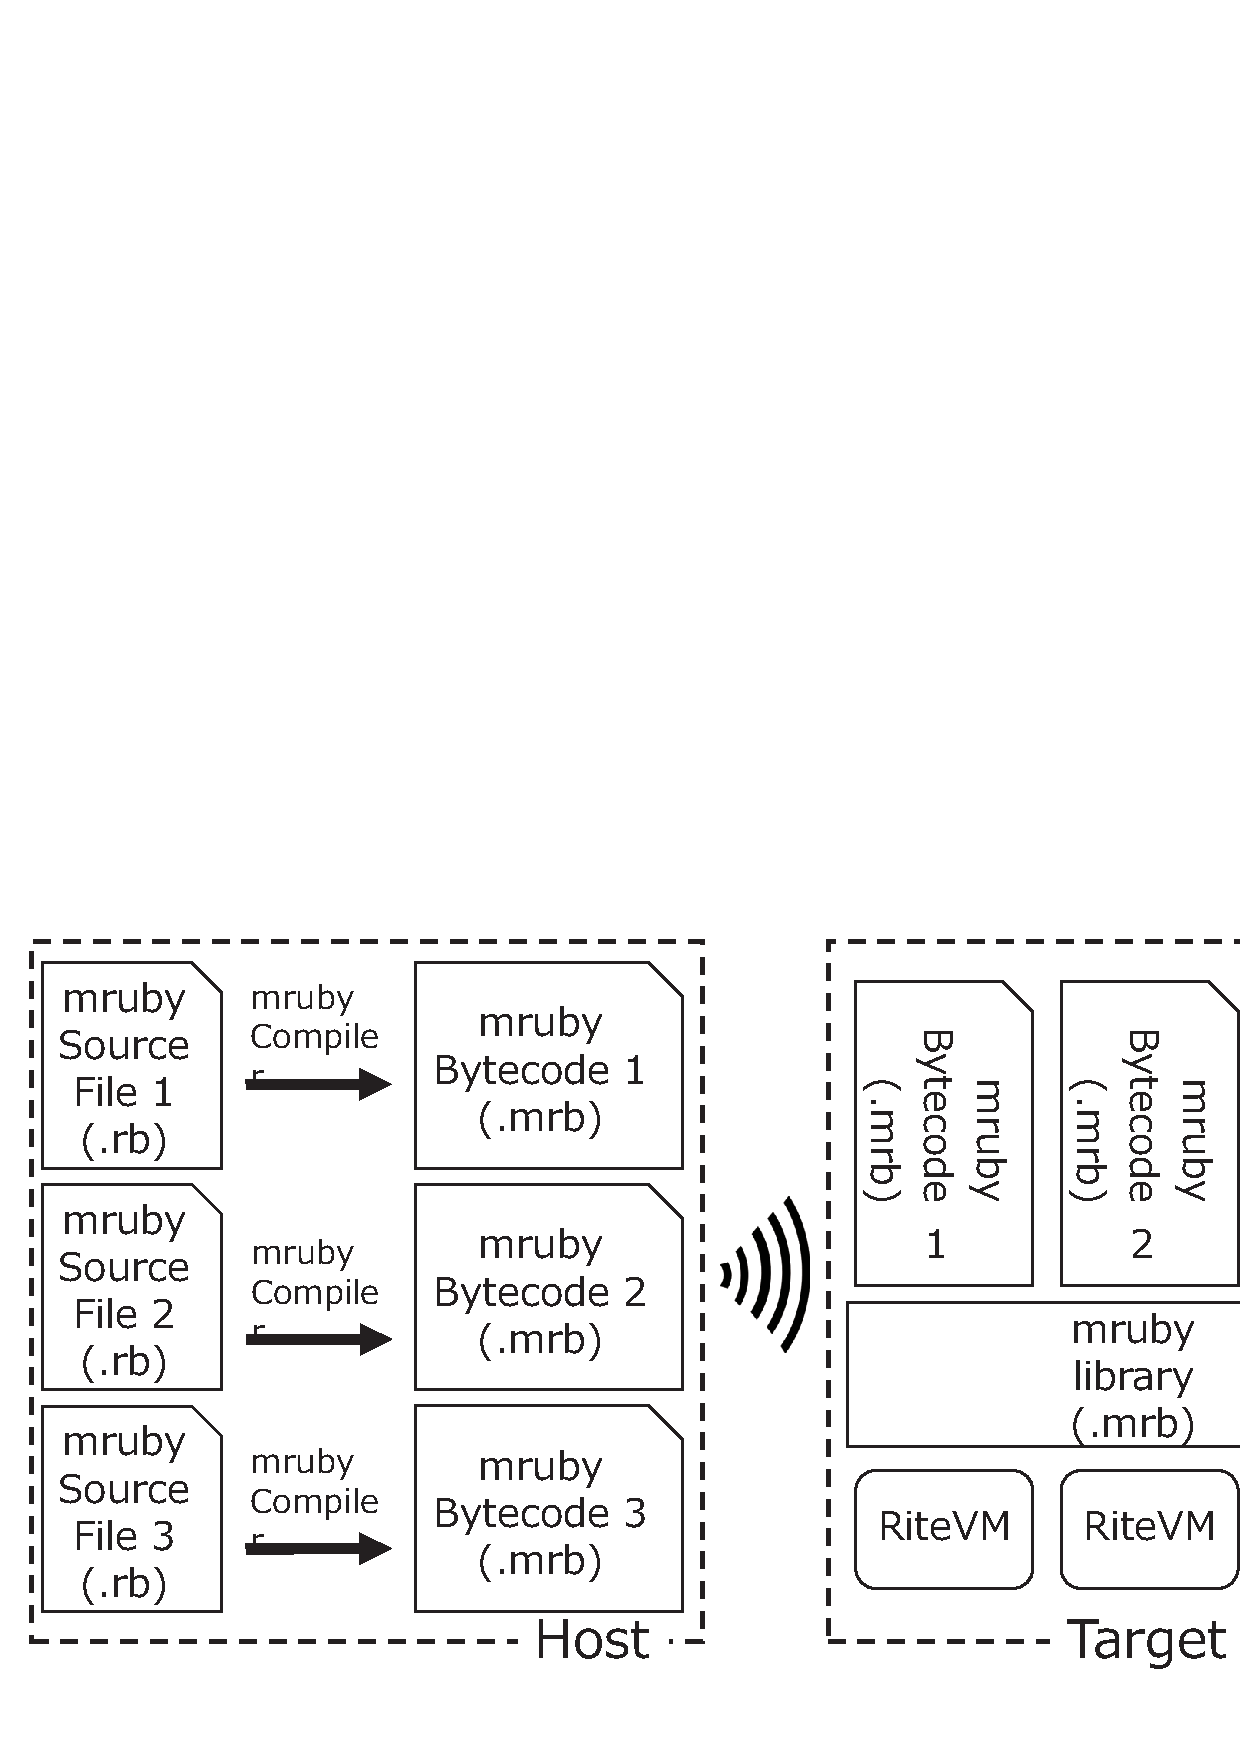
\includegraphics[width=8cm,clip]{../EMSOFT2016/figure/proposed.pdf}
    \caption{System Model}
    \label{fig:proposed}
\end{figure}

\subsection{mruby}
mrubyは,ISO規格の一部に準拠したRubyの軽量実装である.
Ruby\cite{url:Ruby}は,オブジェクト指向型のスクリプト言語である.
特徴としてシンプルな文法なため読みやすくかつ使いやすい上に,C言語よりも少ないコード量で記述できる.
他にも,クラスやメソッドといったオブジェクト指向関数,例外,ガベージコレクションなどの機能により,生産性を向上させることができる.

mrubyは,Rubyの可読性や使いやすさはそのままに,リソースが少なく起動が速いため,組込みシステムに適している.
mrubyには,RiteVMと呼ばれるVMが実装されているため,どのOS上でもアプリケーションを起動させることができる.
図\ref{fig:mruby}にRiteVMのメカニズムを示す.
mrubyコンパイラは,mrubyプログラム(.rb)を,中間言語であるバイトコード(.mrb)にコンパイルする.
RiteVMが実装されいれば,どのターゲットデバイス上でも同じmrubyプログラムを実行できる.

\begin{figure}[t]
    \centering
    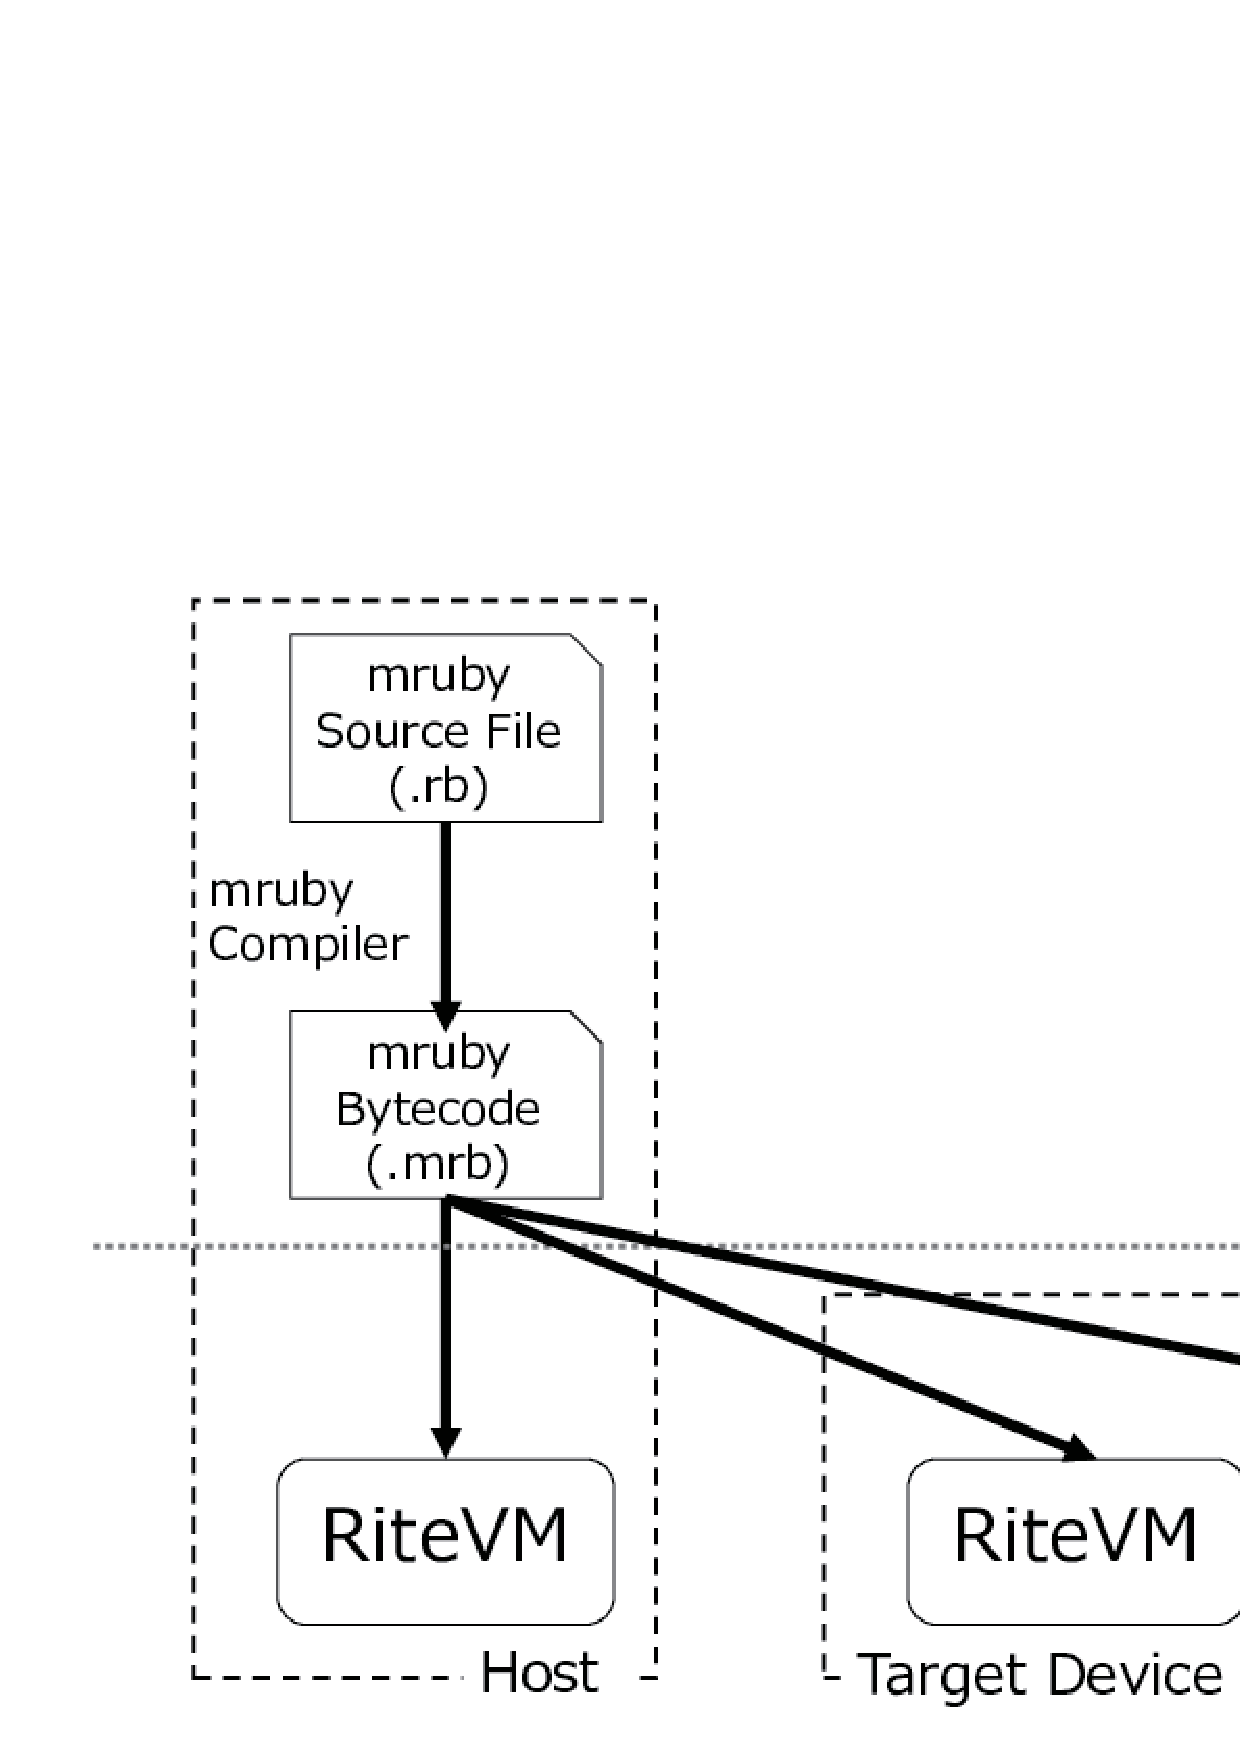
\includegraphics[width=8cm,clip]{../EMSOFT2016/figure/mruby.pdf}
    \caption{Mechanism of mruby/RiteVM}
    \label{fig:mruby}
\end{figure}

\subsection{TECS}
TECS (TOPPERS Embedded Component System)は,組込みシステム向けのコンポーネントシステムである.
TECSによるコンポーネントベース開発は,システム全体の構造を可視化するため,システムの複雑さや難しさを減らすことができる.
さらに,ソフトウェアの共通部分はコンポーネントとして扱われるため,開発の重複を減らし,生産性を向上させる.

TECSでのコンポーネントの生成と結合は静的に行われるため,最適化され,実行時間や消費メモリのオーバヘッドは少ない.
他の特徴として,C言語での実装,ソースレベルでの移植性,コンポーネントの粒度が小さいことなどがある.

\subsubsection{Component Model}
図\ref{fig:component}にコンポーネント図の例を示す.
{\it cell} which is an instance of a component in TECS consists of {\it entry} ports, {\it call} ports, attributes and internal variables.

A {\it entry} port is an interface to provide functions with other {\it cell}s, and a {\it call} port is an interface to use functions of other {\it cell}s.
A {\it cell} has one or more {\it entry} ports and {\it call} ports.
Functions of a {\it cell} are implemented in the C language.

A type of a {\it entry}/{\it call} port is defined by a {\it signature} which is a set of functions.
A {\it signature} is the interface definition of a {\it cell}.
The {\it call} port of a {\it cell} can be connected to the {\it entry} port of another {\it cell} with the same {\it signature}.
A {\it celltype} is the definition of a {\it cell}.
{\it Celltype} defines one or more {\it call}/{\it entry} ports, attributes and internal variables.

\begin{figure}[t]
    \centering
    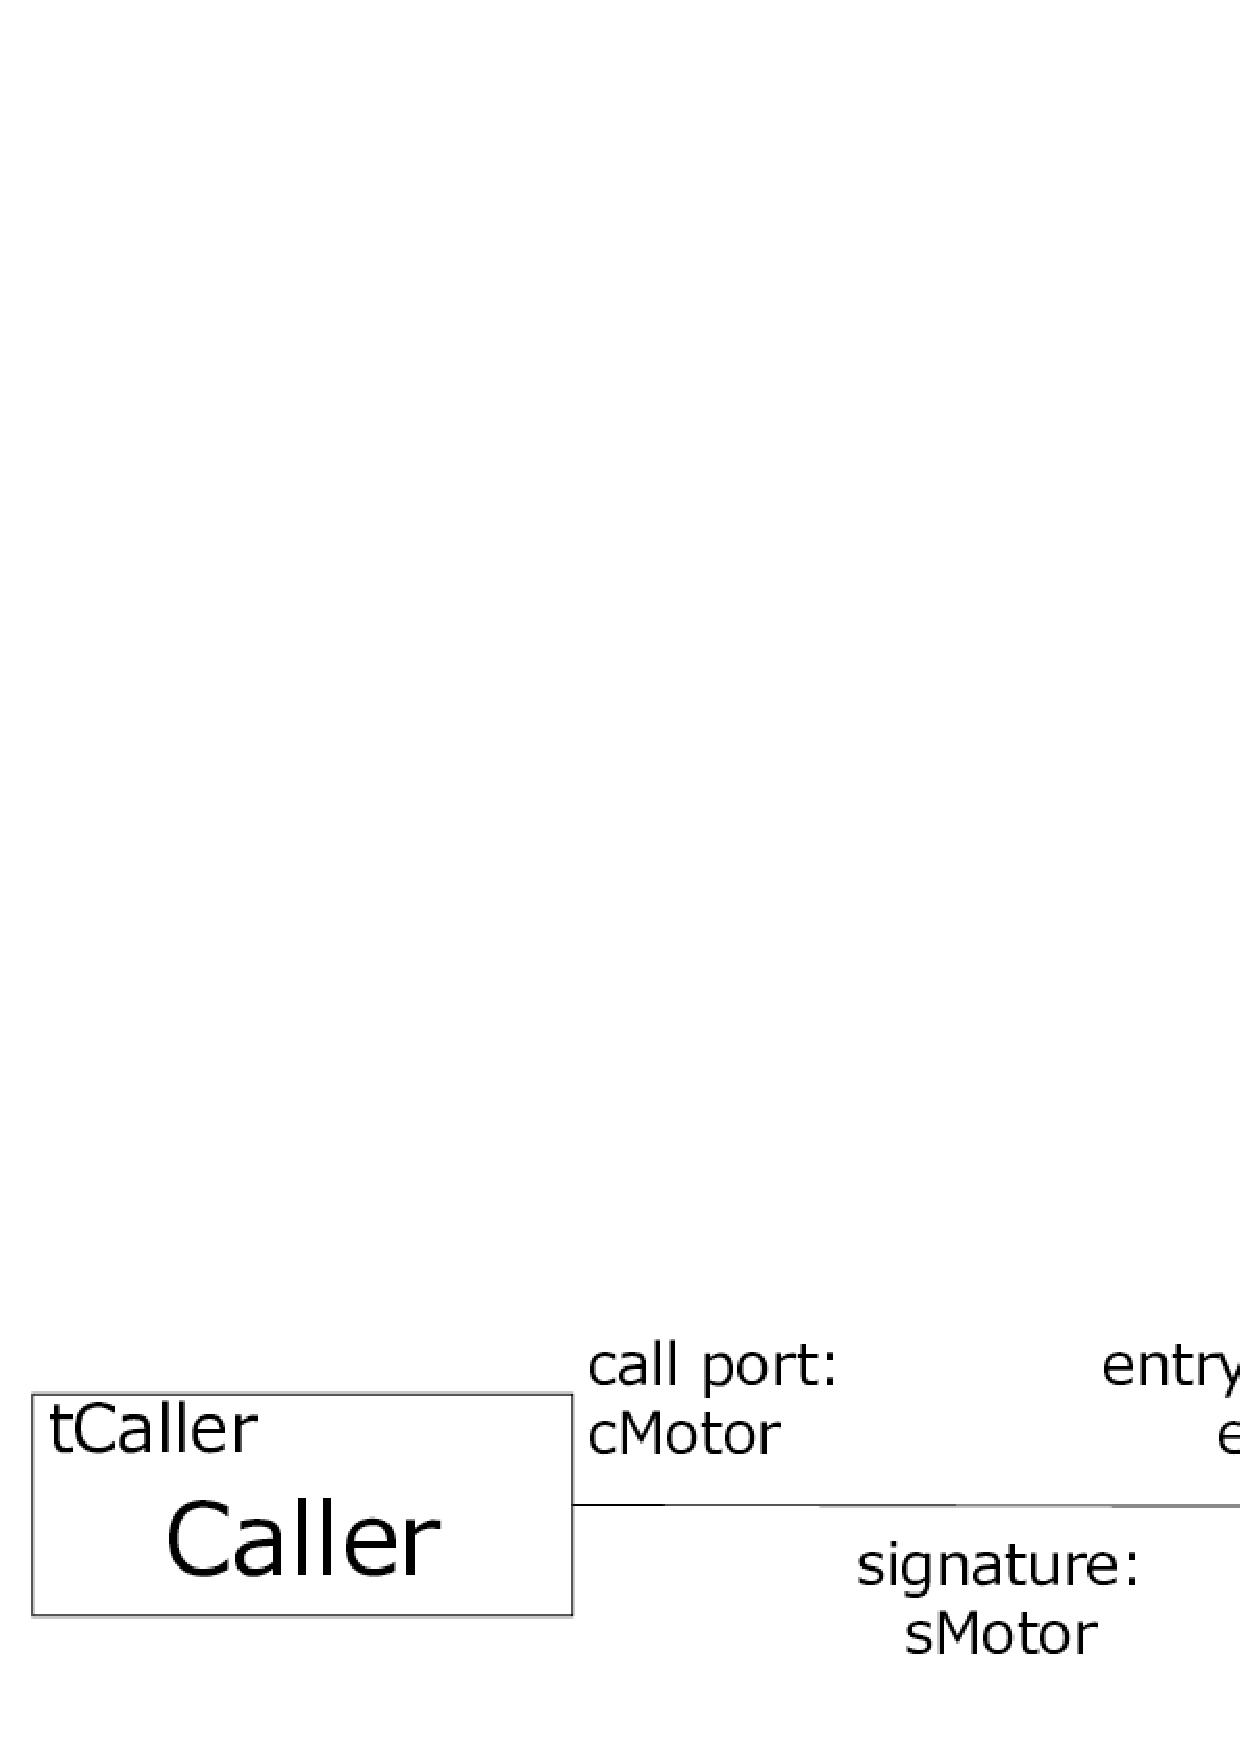
\includegraphics[width=8cm,clip]{../EMSOFT2016/figure/component_diagram.pdf}
    \caption{Component Diagram}
    \label{fig:component}
\end{figure}

\subsubsection{Component Description}
The description of a component in TECS is divided into three parts, {\it signature}, {\it celltype}, and build description.
TECS code is written in .cdl (component description language) file.
The component description is mentioned with an example shown in Figure \ref{fig:component} as follow.

\begin{description}
    \item[{\bf Signature Description}]\mbox{}\\
        The {\it signature} description defines an interface of a {\it cell}.
        A {\it signature} name is described following the keyword {\it signature}.
        It also has the prefix ``s".
        In this way, a {\it signature} is defined such as sMotor shown in Figure \ref{signature}.
        To make the definition of an interface clear, specifiers such as in and out are used in TECS.
        [in] and [out] represent input and output, respectively.\\
\begin{figure}[t]
\centering
\begin{lstlisting}
signature sMotor{
    int32_t getCounts( void );
    ER resetCounts( void );
    ER setPower( [in]int power );
    ER stop( [in] bool_t brake );
    ER rotate( [in] int degrees, [in] uint32_t speed_abs,
              [in] bool_t blocking );
    void initializePort( [in]int32_t type );
};
\end{lstlisting}
\caption{Signature Description}
\label{signature}
\end{figure}

    \item[{\bf Celltype Description}]\mbox{}\\
        The {\it celltype} description defines {\it entry} ports, {\it call} ports, attributes, and valuables of a {\it celltype}.
        An example of a {\it celltype} description is shown in Figure \ref{celltype}.
        A {\it celltype} name following the keyword {\it celltype} with the prefix ``t" and elements of a {\it celltype} is described.
        To define {\it entry} ports, a {\it signature} such as sMotor, and an {\it entry} port name such as eMotor follow the keyword {\it entry}.
        In the same way, {\it call} ports can be declared.
        Attributes and valuables follow the keyword {\it attr} and {\it var} respectively.\\
\begin{figure}[t]
\centering
\begin{lstlisting}
celltype tCaller{
    call sMotor cMotor;
};
celltype tMotor{
    entry sMotor eMotor;
    attr{
        int32_t attr = 100;
    };
    var{
        int32_t var;
    };
};
\end{lstlisting}
\caption{Celltype Description}
\label{celltype}
\end{figure}

    \item[{\bf Build Description}]\mbox{}\\
        The build description is used to instantiate {\it cell}s and connect {\it cell}s.
        Figure \ref{build} shows an example of a build description.
        A {\it celltype} name such as tMotor, and a {\it cell} name such as Motor follow the keyword {\it cell}.
        To compose {\it cell}s, a {\it call} port, a {\it signature}, a {\it entry} port in order are described.
        In this example, a {\it entry} port eMotor in a {\it cell} Motor is connected to a {\it call} port cMotor in a {\it cell} Caller.\\
\begin{figure}[t]
\centering
\begin{lstlisting}
cell tMotor Motor{
};
cell tCaller Caller{
    cMotor = Motor.eMotor;
};
\end{lstlisting}
\caption{Build Description}
\label{build}
\end{figure}

\end{description}

\subsection{mruby on TECS}
\label{sec:mruby on TECS}
mruby on TECS is a component-based framework for running script language.
This framework uses two technologies, mruby and TECS.

\subsubsection{System Model}\mbox{}\\

The system model of mruby on TECS is shown in Figure \ref{fig:mrubyontecs}.
Each mruby program, which is bytecode, runs on its own RiteVM as a componentized task of an RTOS.
TECS components support various embedded drivers such as motor and sensor drivers.

An mruby-TECS bridge plays a role to call a native program (e.g. C legacy code) from an mruby program.
The mruby-TECS bridge provides native libraries for mruby.
It also gives TECS components to receive the invocation from an mruby program.
The mruby-TECS bridge is described in more detail bellow.

As the target RTOS, TOPPERS/HRP2 \cite{url:HRP2}, \cite{par:hr-tecs} is used in this paper.
TOPPERS/HRP2 is an RTOS based on $\mu$ITRON \cite{par:microITRON} with memory protection.
However, mruby on TECS does not depend on the RTOS because TECS supports not only TOPPERS/HRP2 but also the other RTOSs such as OSEK \cite{par:OSEK} and TOPPERS/ASP \cite{url:ASP}.

\begin{figure}[t]
    \centering
    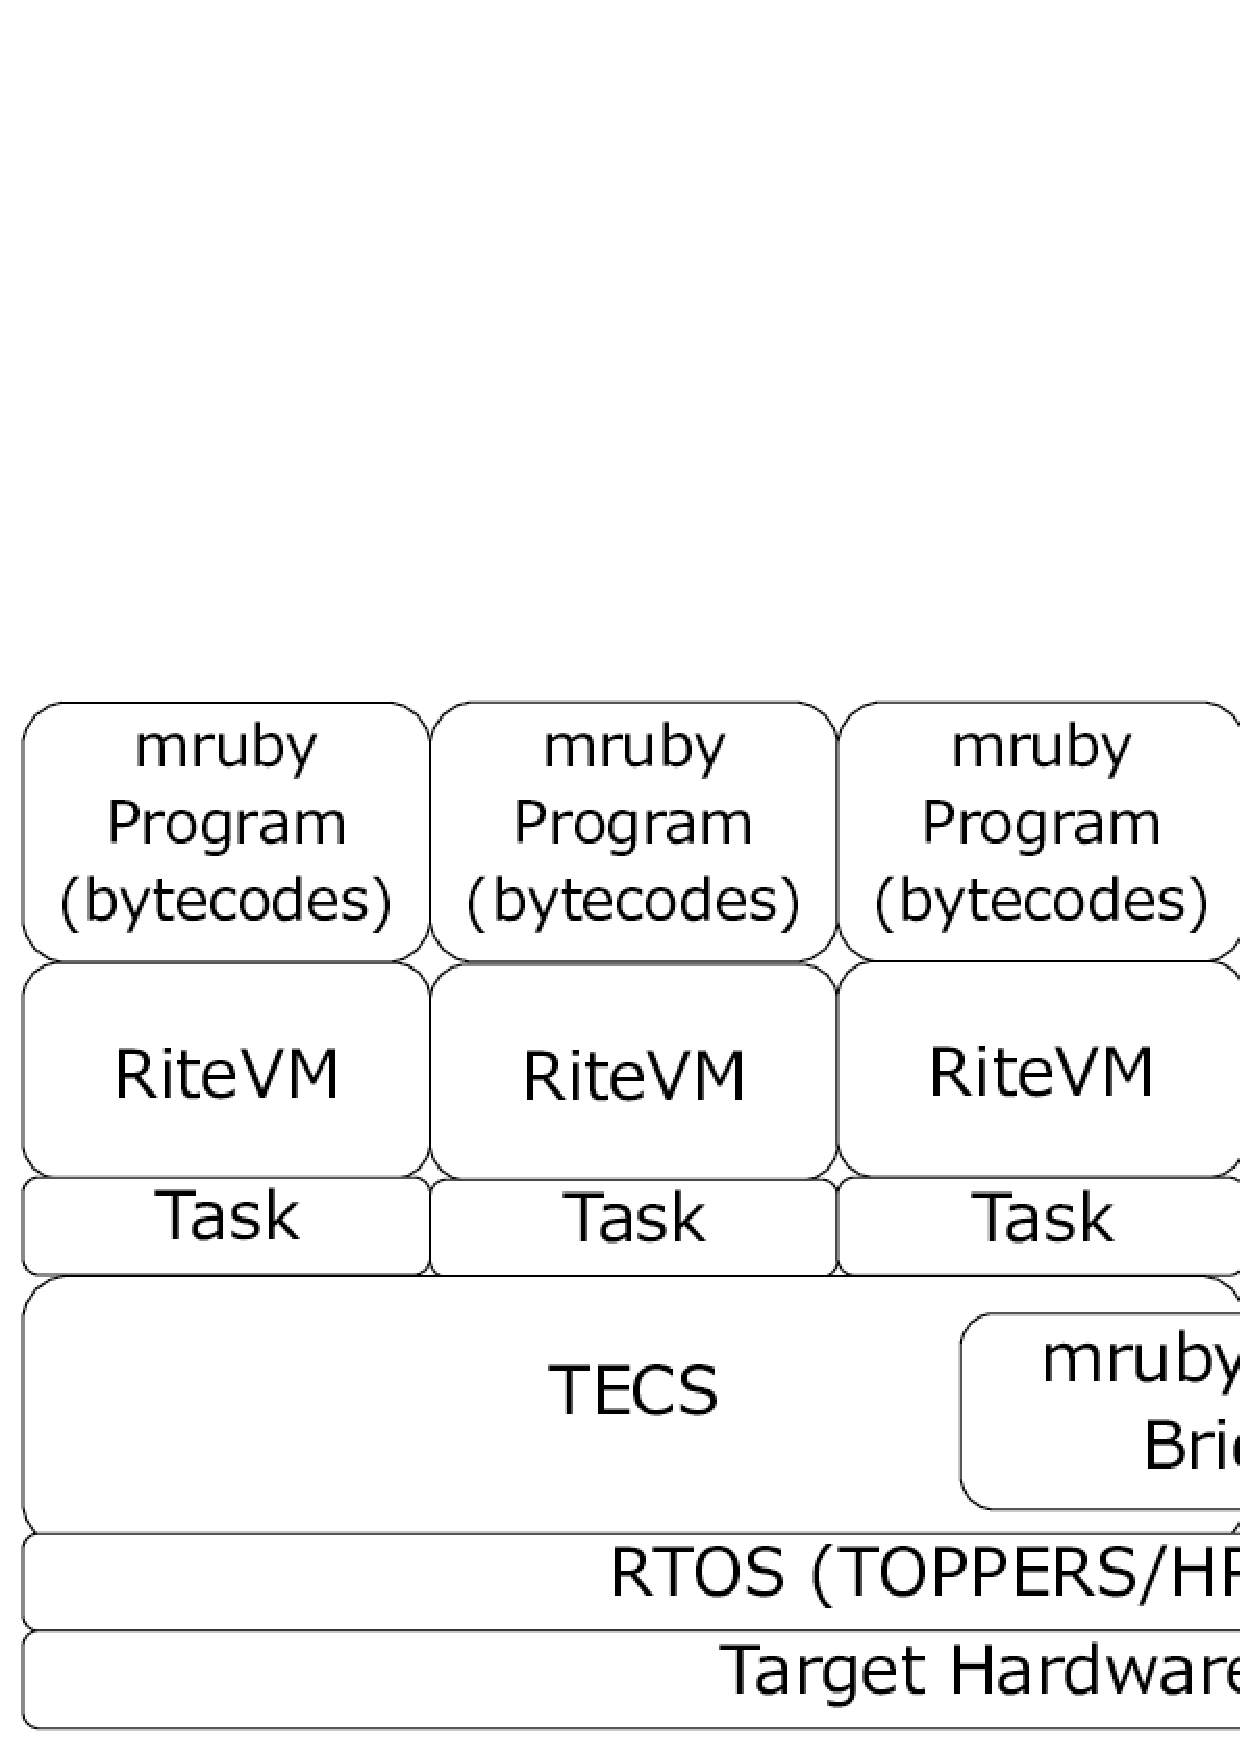
\includegraphics[width=8cm,clip]{../EMSOFT2016/figure/mrubyontecs.pdf}
    \caption{System Model of existing mruby on TECS}
    \label{fig:mrubyontecs}
\end{figure}

\subsubsection{mruby-TECS Bridge}\mbox{}\\

There is a great difference between the execution time of mruby and C language.
According to  \cite{par:mrubyonTECS}, mruby programs are several hundreds times slower than C programs.
The execution of mruby bytecode on a RiteVM is not as efficient as that of C language.
Thus it is difficult to use mruby for all of code.

The use of Ruby on embedded devices provides the benefit of productivity and maintainability due to the ease to use and read.
On the other hands, it is necessary to implement parts of applications in C language in order to manipulate actuators and sensors, and also make a critical section of code run quickly.

Figure \ref{fig:mruby_TECS_bridge} shows an example of use of an mruby-TECS bridge for controlling a motor.
The left side of BridgeMotor belongs to the mruby program.
The right side of BridgeMotor belongs to TECS component.
\begin{figure}[t]
    \centering
    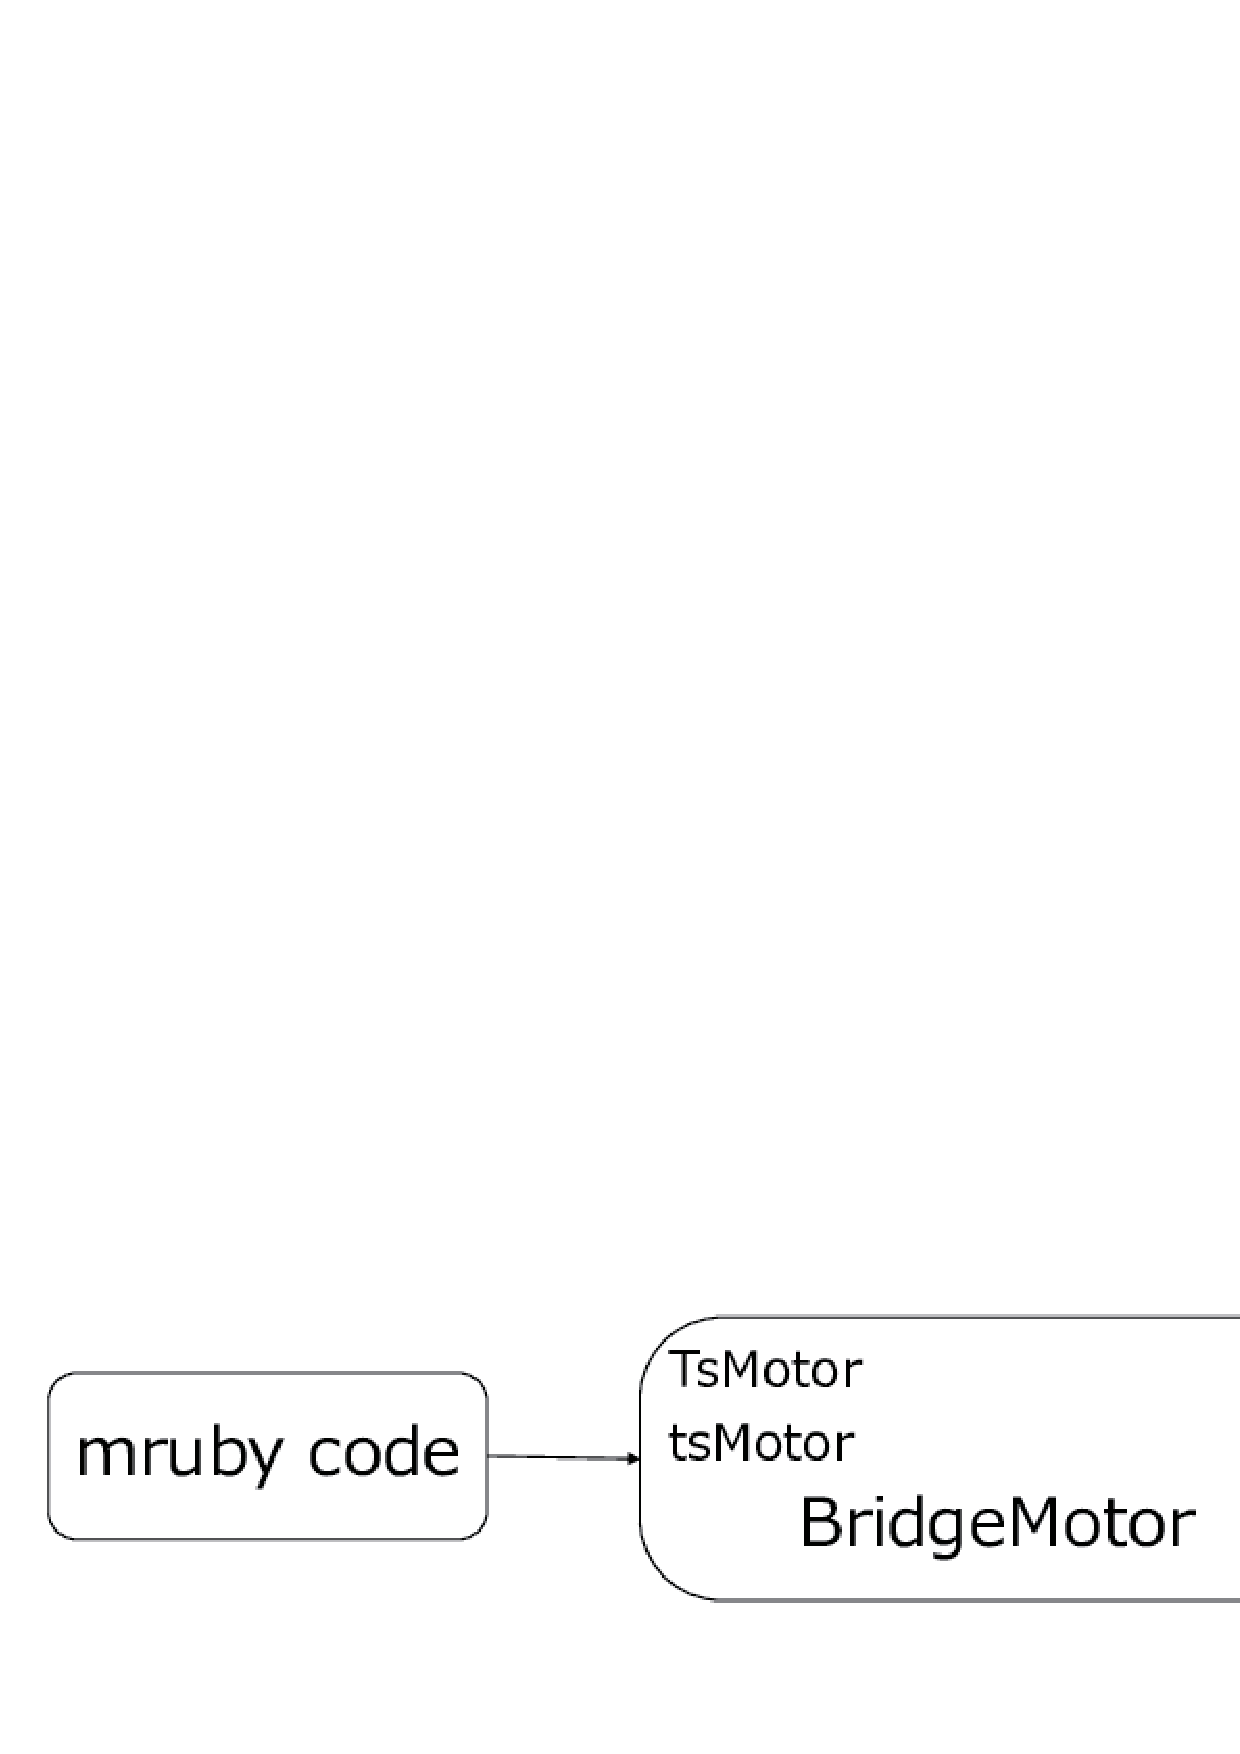
\includegraphics[width=8cm,clip]{../EMSOFT2016/figure/mruby_TECS_bridge.pdf}
    \caption{mruby-TECS Bridge}
    \label{fig:mruby_TECS_bridge}
\end{figure}

The mruby-TECS bridge generates two things.
One is a {\it celltype} to receive invocation from the mruby program.
The other thing is an mruby class that corresponds to the TECS component specified by the developers to invoke a C function from the mruby program.

A code of an mruby-TECS bridge is generated.
The generation code supports registration of classes and methods for mruby.
The methods in an mruby class are defined by generation codes for an mruby-TECS bridge, such as setPower and stop.
Thus, when a method is called in an mruby program, an mruby-TECS bridge calls the function defined in the TECS component such as a Motor {\it cell}.

\section{Design and Implementation}
\label{sec:Design and Implementation}
図\ref{fig:system_model}に提案フレームワークの詳細なシステムモデルを示す.
ホストから転送されたmrubyアプリケーションのバイトコードは,それぞれのRiteVMに実装されたローダで受信され,同期処理により同時に実行される.
RiteVMスケジューラがタスクを周期的に切り替えるため,mrubyアプリケーションは並行動作することができる.
 
Figure \ref{fig:system_model} shows the detailed system model of the proposed framework.
Each mruby application bytecode transferred from the host is received by the loader in the RiteVM.
The RiteVM reads the own bytecode and executes it.
The mruby applications run at the same time because of synchronization processing.
The RiteVM scheuler switches tasks as multiple tasks can run in concurrent.

\begin{figure}[t]
    \centering
    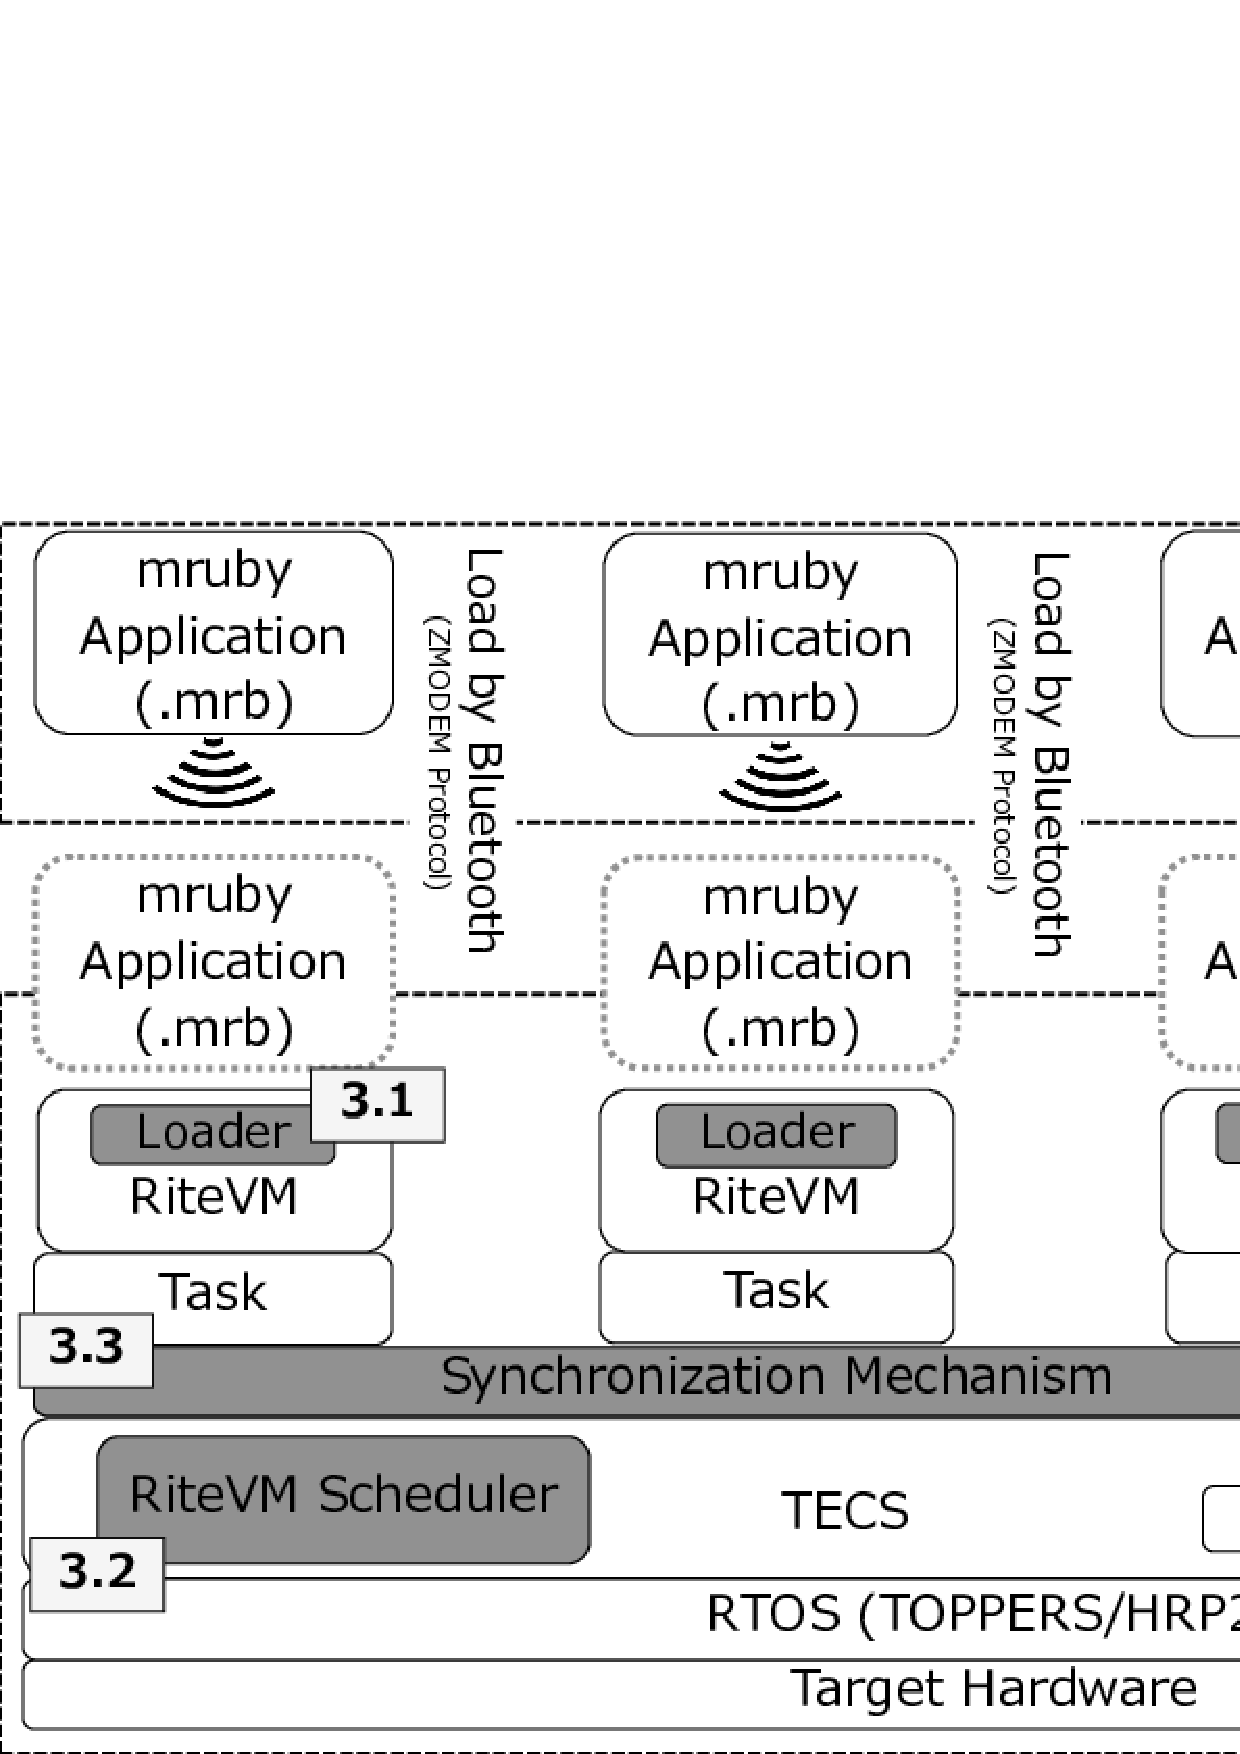
\includegraphics[width=8cm,clip]{../EMSOFT2016/figure/system_model.pdf}
    \caption{Detailed System Model of the proposed framework}
    \label{fig:system_model}
\end{figure}

\subsection{mruby Bytecode Loader Using Bluetooth}
\label{sec:mruby bytecode loader using Bluetooth}
この章では,Bluetoothを用いたmrubyバイトコードローダについて述べる.
現状のmruby on TECSでは,mrubyバイトコードをプラットフォームに組み込んでいるため,mrubyプログラムを修正する度にプラットフォーム部分をもう一度コンパイル・リンクし,SDカードやROMといったデバイスに再度書き込み,OSを再起動する必要がある.
このような作業を繰り返すことで,作業効率は悪くなる.
提案フレームワークでは,プラットフォーム部分をコンパイル・リンクし記憶デバイスに書き込むのは,はじめの一度だけで良いため,作業効率を向上させることができる.

mrubyプログラムは,アプリケーション部分とライブラリ部分に分けられる.
mrubyアプリケーションは,開発者が主にプログラムするメインのコードであり,mrubyライブラリには,motorクラスやsensorクラスといったRubyクラスのようにアプリケーションで利用される関数群が定義されている.
アプリケーションとライブラリを含んだmrubyバイトコードを転送し,実行することもできるが,提案フレームワークでは,ライブラリ部分はプラットフォームに組込み,アプリケーション部分のみを転送する設計にした.
このような設計にすることで,ライブラリは頻繁に変更されないため,毎回コンパイルする無駄を省くことができる.
さらに,各RiteVMでライブラリを共有することや,RiteVM固有のライブラリを持つことも可能になる.

提案フレームワークでは,mrubyバイトコードの連続ローディングにも対応している.

\subsubsection{Component of RiteVM with mruby bytecode loader using Bluetooth}
提案フレームワークでは,mrubyバイトコードローダはTECSのコンポーネントとして提供されている.
このコンポーネントは,RiteVMのコンポーネントの拡張として実装されている.(詳細については\cite{par:mrubyonTECS}を参照)
このコンポーネントでは,転送されたバイトコードの受信に加え,RiteVMのコンフィグレーションが行われる.

図\ref{fig:component_bluetooth}に,MrubyTask1とMrubyBluetooth1のコンポーネントの例を示す.
MrubyTask1は,コンポーネント化されたRTOS (TOPPERS/HRP2 \ref{url:HRP2}\ref{par:HRP2})のタスクである.
MrubyBluetooth1は,mrubyバイトコードを実装したRiteVMのコンポーネントであり,このコンポーネントのはじめで転送されてきたバイトコードを受信する.
提案フレームワークでは,バイナリ転送プロトコルとして,ZMODEを適用した.

\begin{figure}[t]
    \centering
    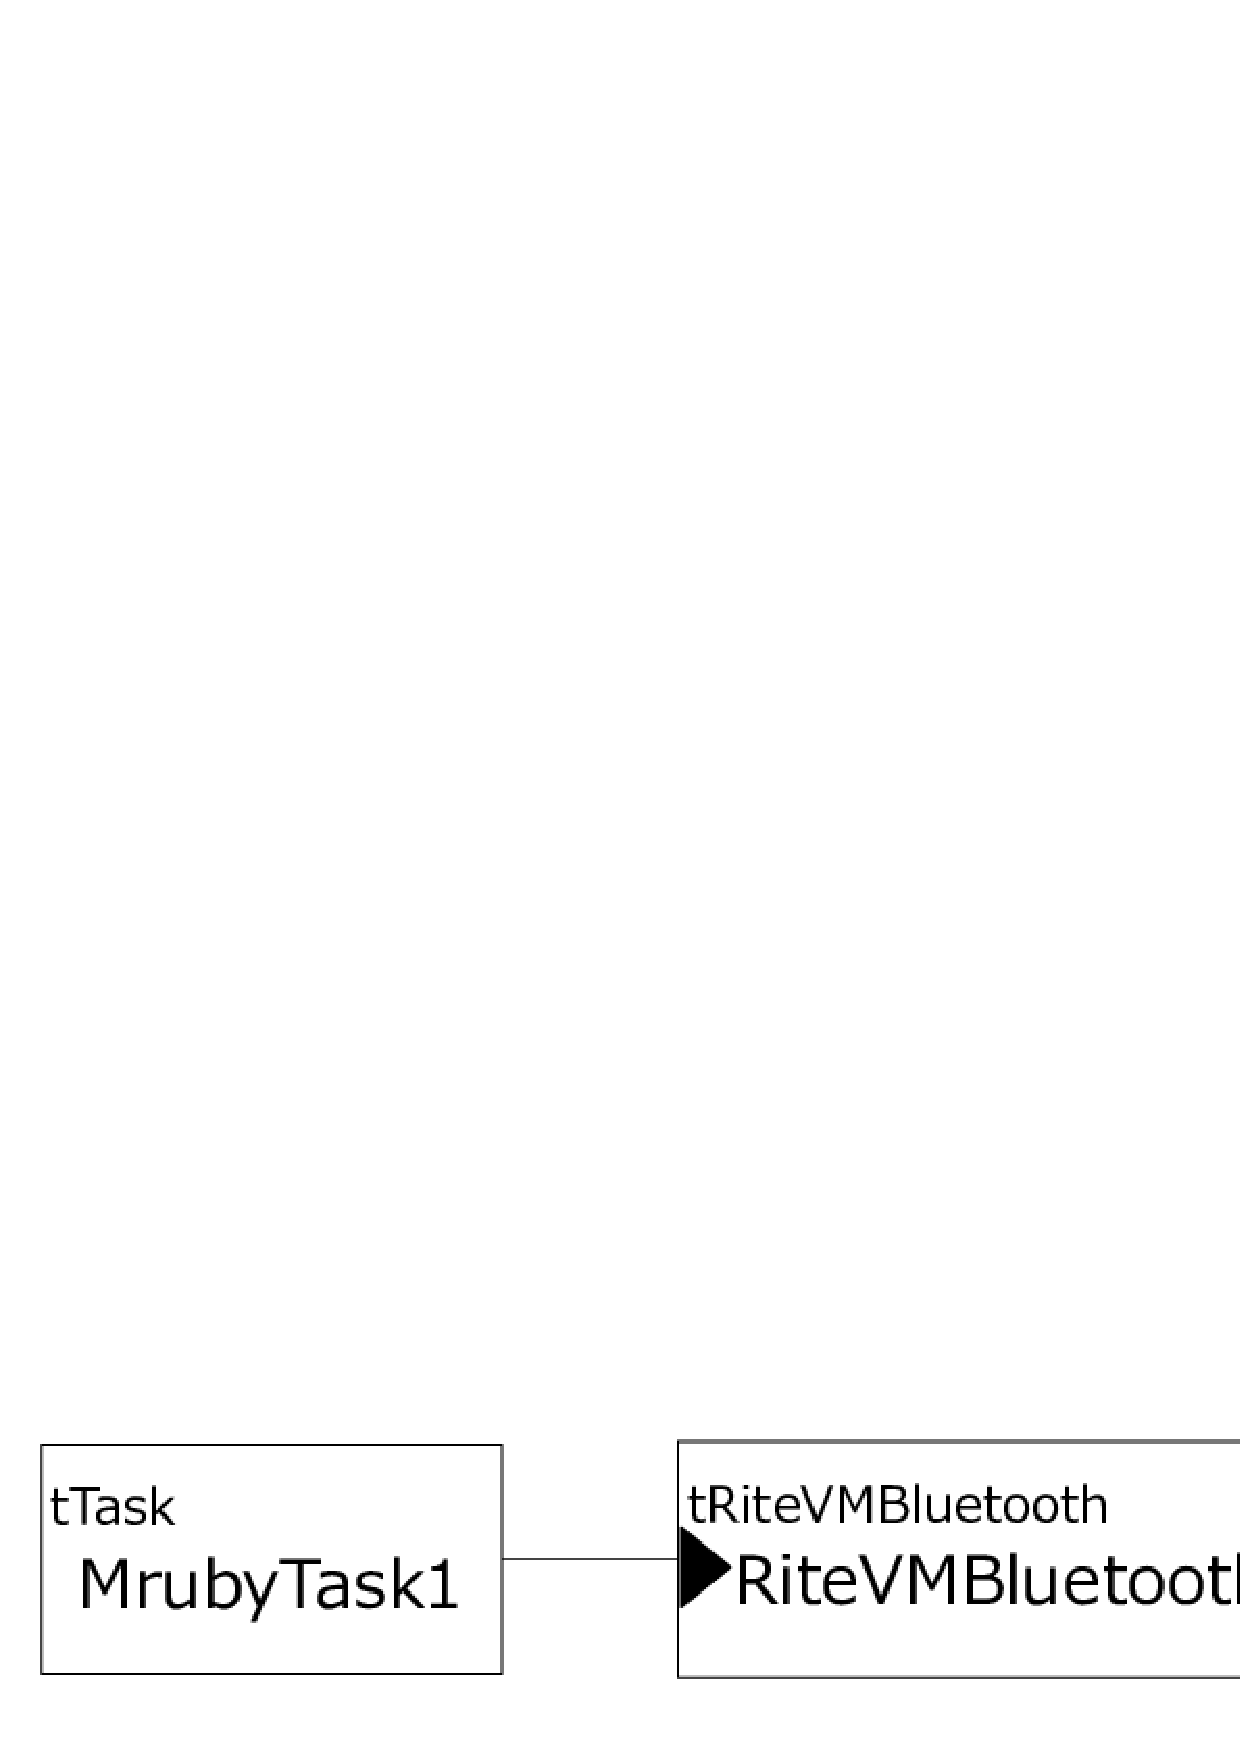
\includegraphics[width=8cm,clip]{../EMSOFT2016/figure/component_bluetooth.pdf}
    \caption{Component Diagram of mruby bytecode loader using Bluetooth}
    \label{fig:component_bluetooth}
\end{figure}

図\ref{fig:control_flow}に,ローダを実装したRiteVMがmrubyプログラムを実行するまでの制御フロー,図\ref{maincode_mrubybluetooth}には,RiteVMコンポーネントのソースコードを示す.

はじめに,{\it mrb\_state}と{\it mrbc\_context}のポインタを初期化する.
{\it mrb\_state}は,mrubyで使われる状態と変数のセットである.

次に,mrubyライブラリのバイトコードを読み込む.
図\ref{celltype_mrubybluetooth}に示すように,tMrubyBluetoothのセルは属性を持っている.
{\it mrubyFile}はmrubyライブラリのファイルを示しており,{\it [omit]}はTECSジェネレータによってのみ使えわれるため,この属性はメモリを消費することない.
{\it irep}は,mrubyライブラリのバイトコードが格納されている配列へのポインタである.
つまり,mrubyライブラリは始めのコンパイル時にコンポーネントの属性として,配列に保存されている.

次に,転送されてきたmrubyアプリケーションのバイトコードを読み込む.
mrubyアプリケーションのバイトコードは,図\ref{celltype_mrubybluetooth}に示す,内部変数uint8\_t型の配列{\it irepApp}に格納されている.
2つのバイトコードは,それぞれ別の配列に保存されており,別々に読み込まれる.

最後に,RiteVMはmrubyアプリケーションであるタスクを実行する.
mrubyアプリケーションのプログラムが修正された場合は,そのバイトコードのみを再転送する.

\begin{figure}[t]
    \centering
    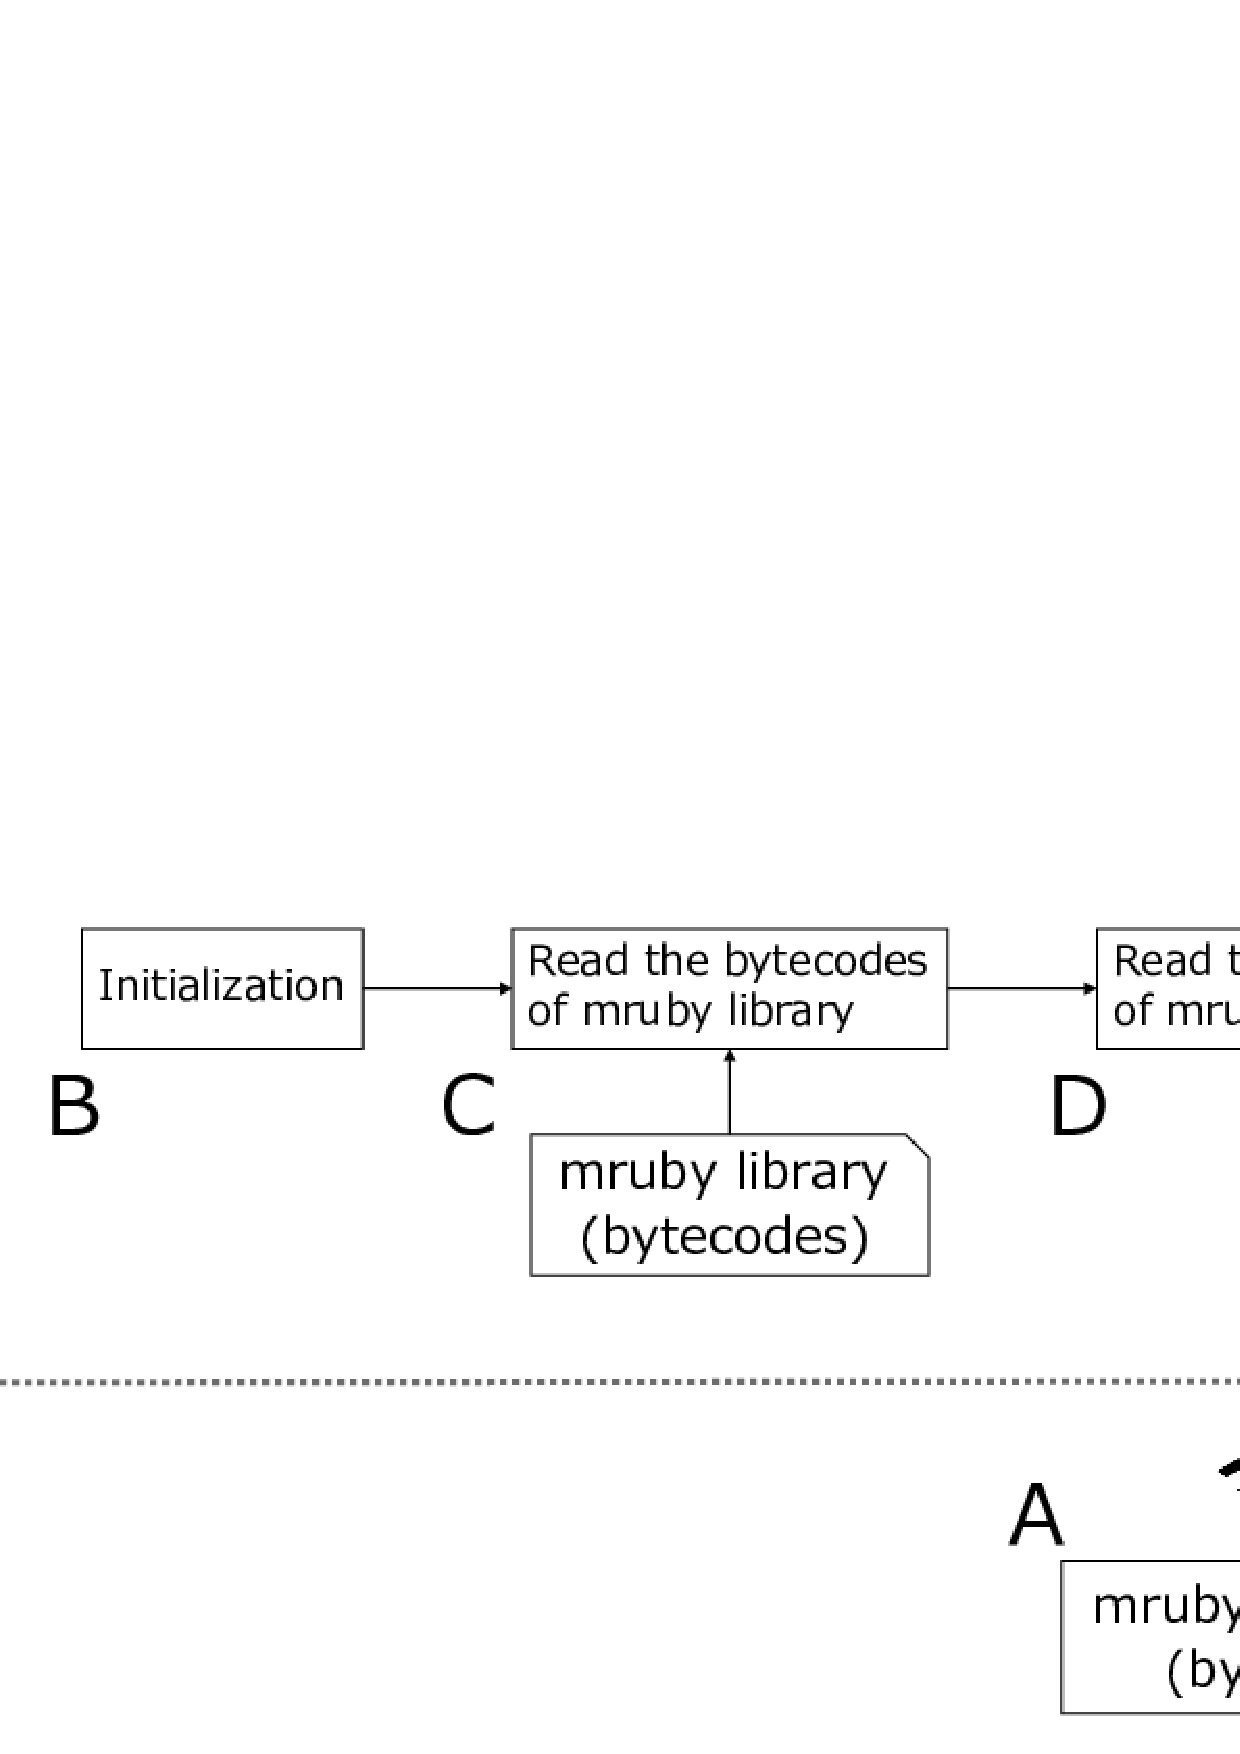
\includegraphics[width=8cm,clip]{../EMSOFT2016/figure/control_flow.pdf}
    \caption{Control Flow of mruby bytecode loader using Bluetooth}
    \label{fig:control_flow}
\end{figure}
\begin{figure}[t]
\centering
\begin{lstlisting}
celltype tMrubyBluetooth{
    entry sTaskBody eMrubyBody;
    attr{
      [omit]char_t *mrubyFile;
      char_t *irep = C_EXP("&$cell_global$_irep");
      uint32_t irepAppSize = C_EXP( BUFFER_SIZE );
    };
    var{
        [size_is(irepAppSize)] uint8_t *irepApp;
    };
};
\end{lstlisting}
\caption{Celltype Description for RiteVM with mruby bytecode loader using Bluetooth}
\label{celltype_mrubybluetooth}
\end{figure}
\begin{figure}[t]
\centering
\begin{lstlisting}
void
eMrubyBody_main( CELLIDX idx )
{
  /* Declaration variables */
  mrb_state *mrb;
  mrbc_context *c;
  /* New interpreter instance */
  mrb = mrb_open();
  // Omit: error check for mrb_state
  /* New mruby context */
  c = mrbc_context_new( mrb );
  // Omit: initialization of mruby-TECS bridge
  /* Receive the bytecode via Bluetooth */
  bluetooth_loader( VAR_irepApp );
  /* Load mruby library bytecode and run */
  mrb_load_irep_cxt( mrb, ATTR_irep, c );
  /* Load mruby application bytecode and run */
  mrb_load_irep_cxt( mrb, VAR_irepApp, c );
  if ( mrb->exc ) {
    /* Failure to execute */
    mrb_p( mrb, mrb_obj_value( mrb->exc ) );
    exit( 0 );
  }
  /* Free mruby context */
  mrbc_context_free( mrb, c );
  /* Free interpreter instance */
  mrb_close( mrb );
}

\end{lstlisting}
\caption{Main code for RiteVM with mruby bytecode loader using Bluetooth}
\label{maincode_mrubybluetooth}
\end{figure}
\subsection{Multitask}
\label{sec:Multitask}
この章では,提案フレームワークでのマルチタスク処理の設計にちて述べる.
mruby on TECSは,マルチタスクに対応しているが,開発者がRTOSの知識を熟知している必要がある.

マルチタスク処理のアプローチのひとつにコルーチンがある.
コルーチンは,協調的スレッドであり,開発者が{\it resume}や{\it yield}といった関数を呼び出すことで並列動作を行うことができる.
(Rubyのコルーチンは,Fiberクラスに定義されている.\cite{url:co-routine})
コルーチンは,ノンプリエンプティブな処理で,開発者自身がタスクの切り替えを行う必要があるので,OSのサポートやマルチコアの恩恵を受けることができない.

その他のアプローチとして,μITRONのサービスコールである{\it delay()}使った手法がある.
このサービスコールは,引数として与えられた時間だけ,そのタスクの起動を遅らせる.
{\it delay()}は,固定優先度スケジューリングの場合に用いられるが,フェアスケジューリングの場合には使用することが難しい.

提案フレームワークでは,フェアスケジューラであるRiteVMスケジューラを実装し,複数のタスクを平等に並行動作させる.
このスケジューラはアプリケーションタスクが同じ優先度を持つ場合に利用でき,開発者がOSの関数を呼び出すことなく,マルチタスク処理が可能になる.
その上,既存のアプリケーションプログラムの構造を変えること使うことができる. 

\subsubsection{RiteVM Scheduler}
RiteVMスケジューラは,周期ハンドラであり,μITRONのサービスコールである{\it rotateReadyQueue}を呼び出す.
{\it rotateReadyQueue}は,同優先度のタスクの実行を切り替える関数である.
RiteVMスケジューラの設計を図\ref{fig:rotateReadyQueue}に示す.

無限ループを持った同優先度の2つのタスクの場合を考える.
現状のシステムでは,始めにタスクが起動すると,そのタスクが無限ループに入るため,もう片方のタスクが起動することができない.

{\it rotateReadyQueue}が呼ばれると,図\ref{fig:rotateReadyQueue}に示すように,タスクの起動が切り替わる.
{\it rotateReadyQueue}の引数は,優先度である.

{\it rotateReadyQueue}は,2つ以上のタスクの場合にでも利用できる.
例えば,3つのタスク,task 1, 2, 3が順に起動する場合,{\it rotateReadyQueue}が呼ばれると,task 2, 3, 1の順にタスクの起動は切り替わる.

\begin{figure}[t]
    \centering
    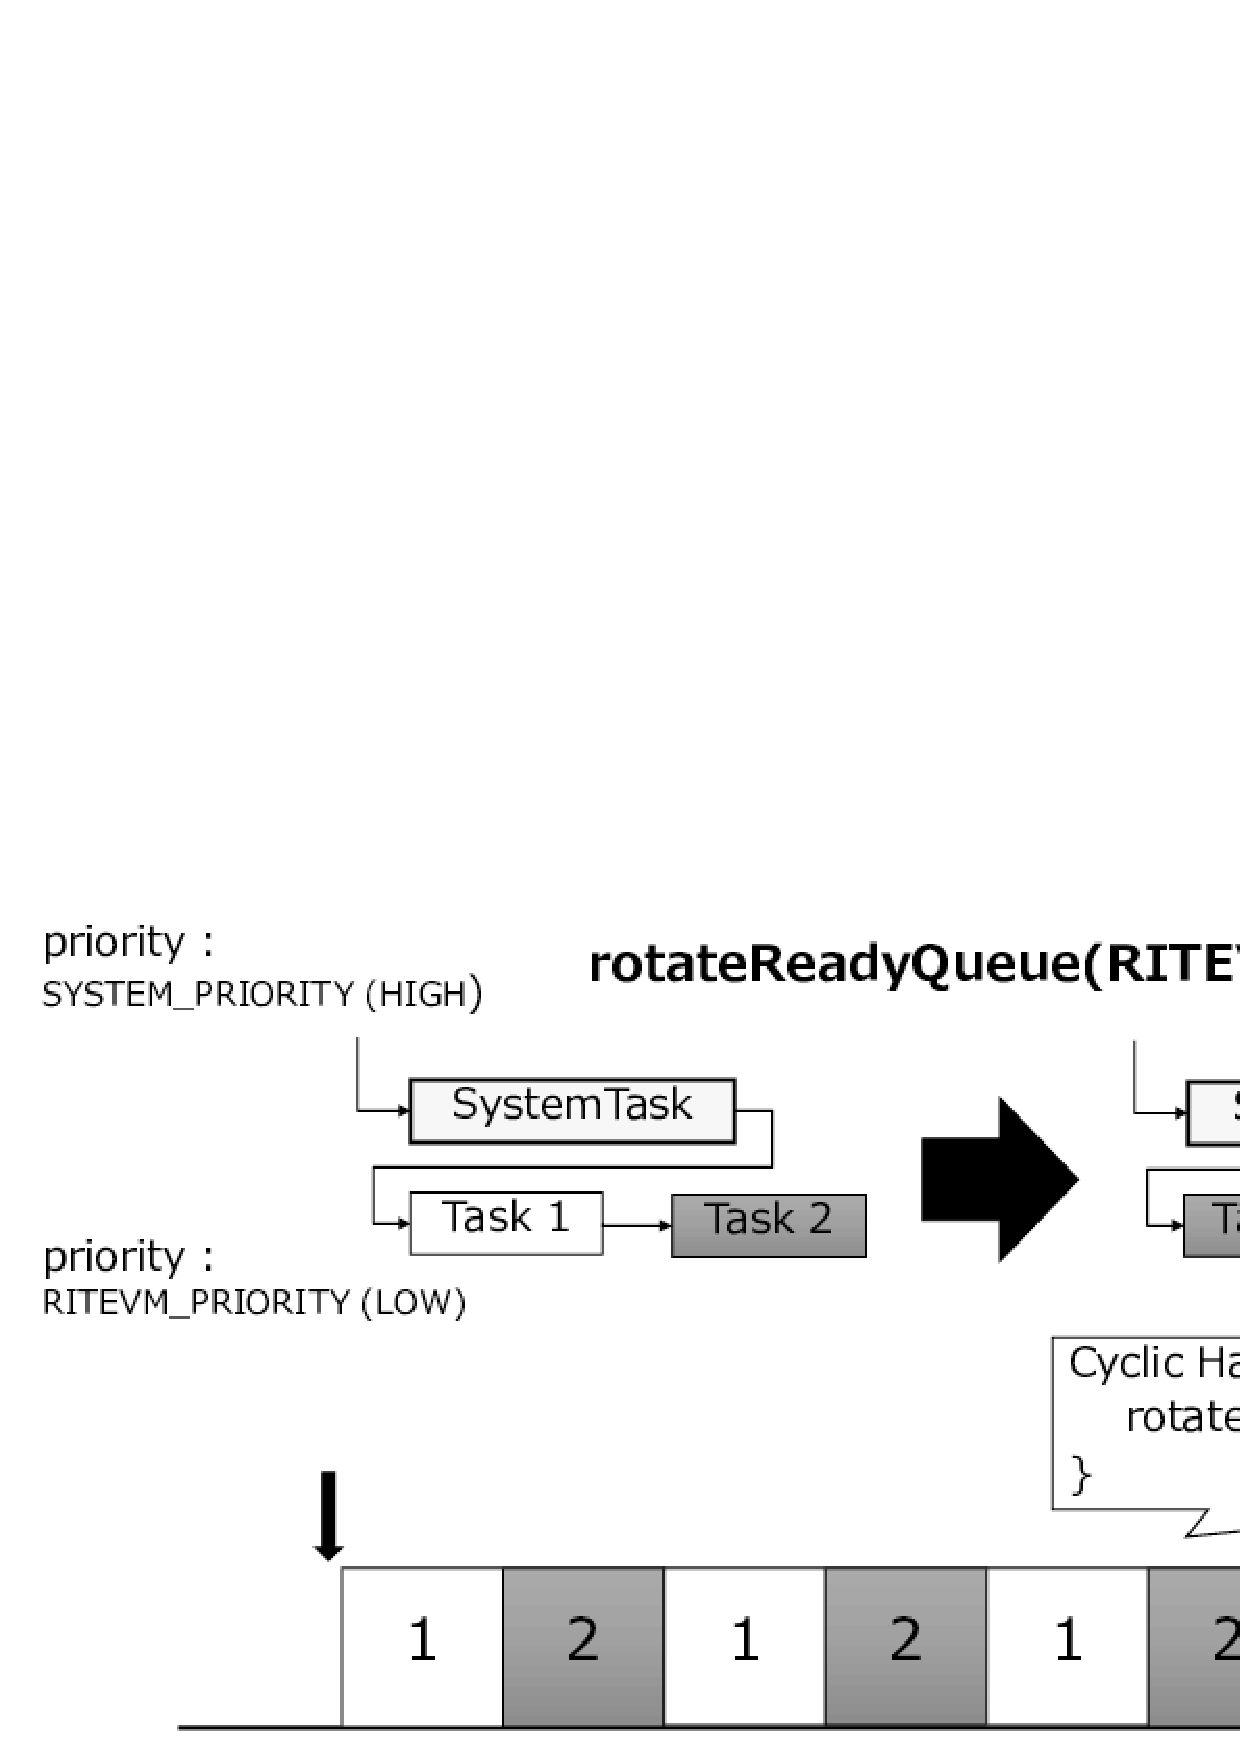
\includegraphics[width=8cm,clip]{../EMSOFT2016/figure/rotateReadyQueue.pdf}
    \caption{The design of RiteVM sceduler}
    \label{fig:rotateReadyQueue}
\end{figure} 
 
\subsubsection{Component of RiteVM Scheduler}
図\ref{fig:cyclic_handler}にRiteVMスケジューラのコンポーネント図を示す.
RiteVMスケジューラのコンポーネントは,CyclicHandlerとCyclicMainから構成される.
CyclicHandlerセルは,μITRONの周期ハンドラの設定を行う.
μITRONの周期ハンドラは,\cite{par:microITRON}に詳しく書かれている.

周期ハンドラは,5つの引数を持っている.(ID, attribute, cyclic time, cyclic phase, access pattern)
CyclicHandlerセルは,3つの引数をセルの属性として持っている.
CyclicMainセルは,周期ハンドラの処理を行うコンポーネントであり,{\it rotateReadyQueue}が実装されている.
図\ref{celltype_cyclic_handler}に,セルタイプtCyclicMainのセルタイプ記述を示す.
{\it call}ポートは,カーネルの機能を使用するためにカーネルセルの{\it entry}ポート({\it tkernel.eiKernel})に接続されている.
属性は,{\it rotateReadyQueue}の引数として使われる.

図\ref{build_cyclic_handler}に,図\ref{fig:cyclic_handler}に示されるコンポーネントの組み上げ記述を示す.

CyclicHandlerセル部分では,cyclicTimeやcyclicPhaseといった属性で与えられる周期ハンドラの設定を行う.
attributeは{\it TA\_STA}であるので,OSが起動すると周期ハンドラが実行状態となる.
周期時間は,1msecである.
CyclicMainセル部分には,属性としてpriorityが記述されている.
RITEVM\_PRIORITYはmrubyタスクの優先度として定義されている.
この属性は,{\it rotateReadyQueue}の引数として与えられる.

\begin{figure}[t]
    \centering
    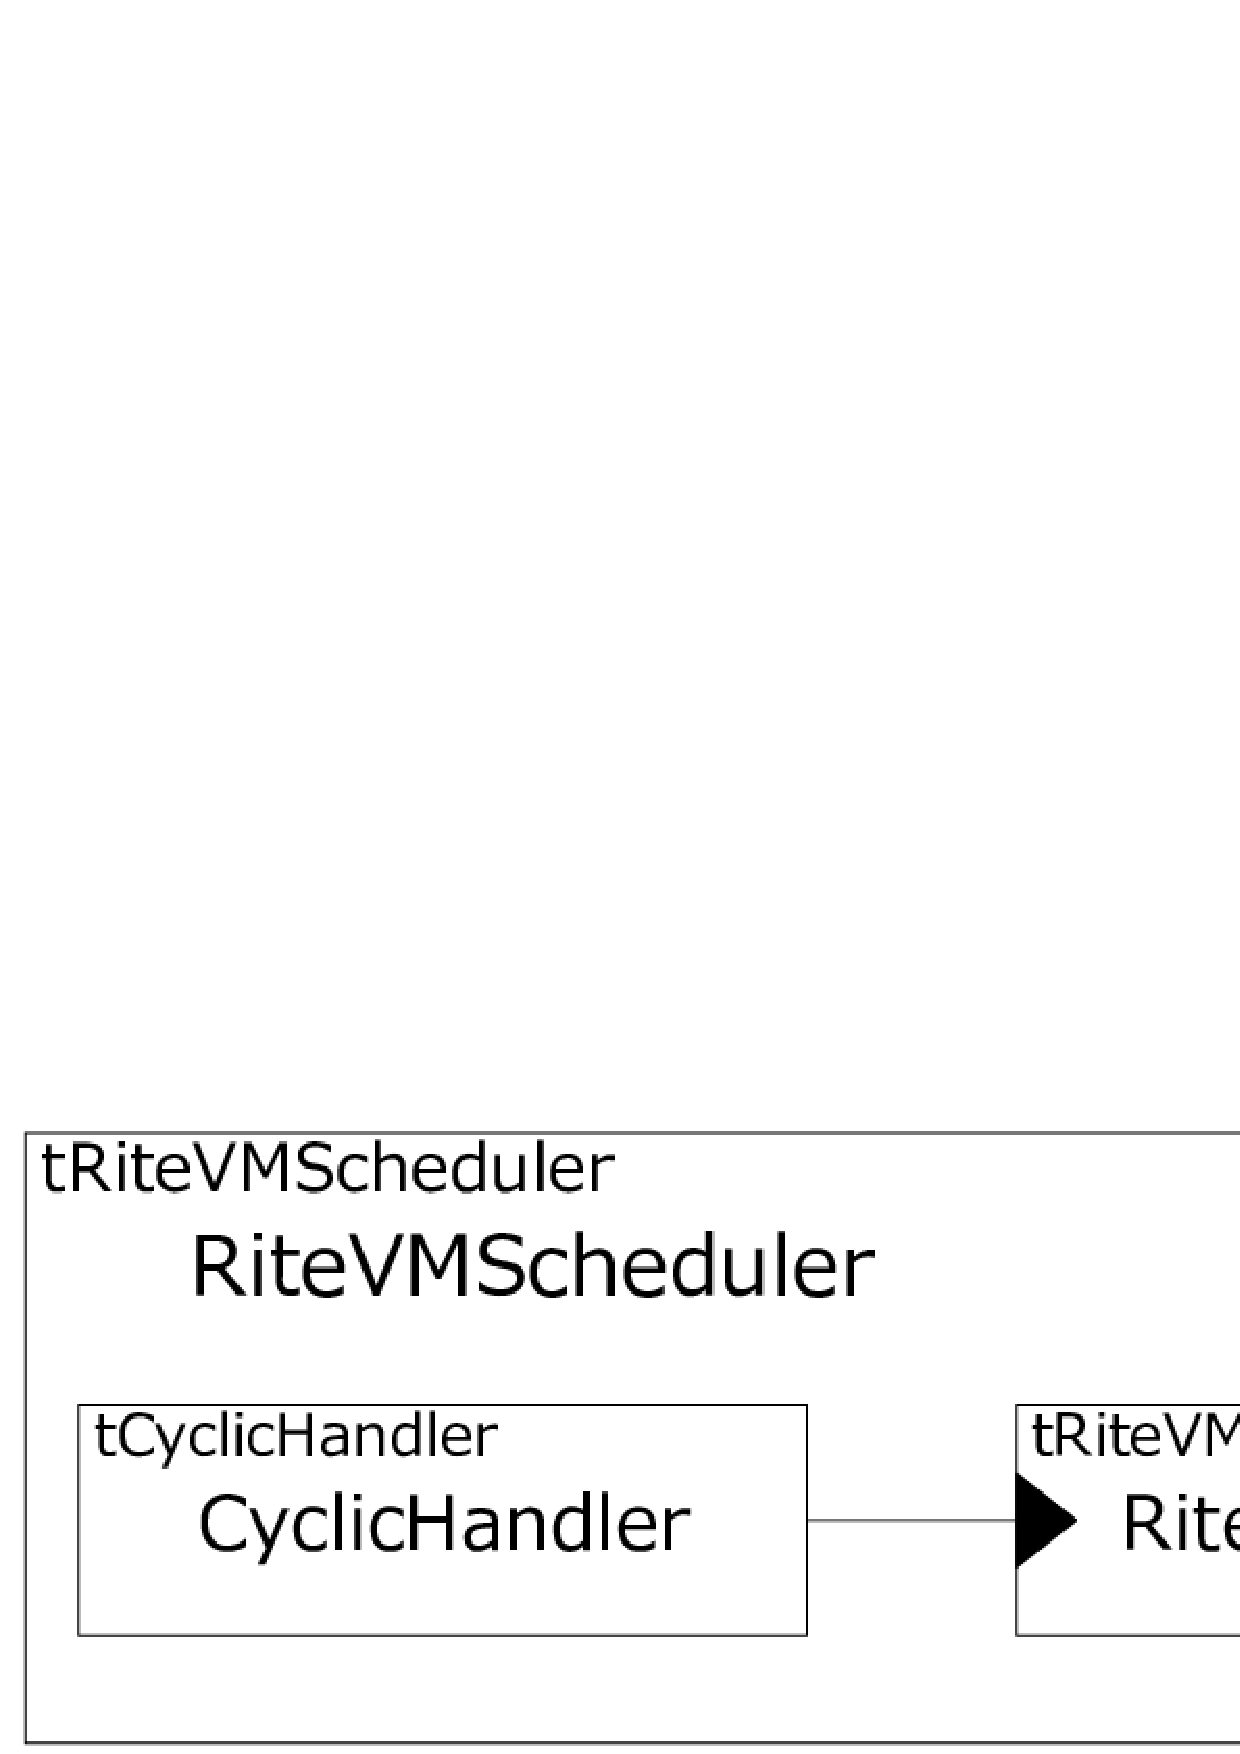
\includegraphics[width=8cm,clip]{../EMSOFT2016/figure/cyclic_handler.pdf}
    \caption{Component Diagram of Cyclic Handler}
    \label{fig:cyclic_handler}
\end{figure}
\begin{figure}[t]
    \centering
    \begin{lstlisting}
celltype tCyclicHandler {
    [inline] entry sCyclic eCyclic;
    call  siHandlerBody  ciBody;
    attr {
    	[omit] ATR    attribute = C_EXP("TA_NULL");
    	[omit] RELTIM cyclicTime;
    	[omit] RELTIM cyclicPhase = 0;
    };
};
celltype tCyclicMain{
    require tKernel.eiKernel;
    entry siHandlerBody eiBody;
    attr {
        PRI priority;
    };
};
    \end{lstlisting}
    \caption{Celltype Description of Cyclic Handler}
    \label{celltype_cyclic_handler}
\end{figure}
\begin{figure}[t]
    \centering
    \begin{lstlisting}
cell tCyclicHandler CyclicHandler{
    ciBody = CyclicMain.eiBody;
    attribute = C_EXP("TA_STA");
    cyclicTime = 1;
    cyclicPhase = 1;
};
cell tCyclicMain CyclicMain{
    priority =
        C_EXP("RITEVM_PRIORITY");
};
   \end{lstlisting}
    \caption{Build Description of Cyclic Handler}
    \label{build_cyclic_handler}
\end{figure}
 
\subsubsection{Synchronization of Multiple RiteVM Tasks}
複数のmrubyアプリケーションの起動を同期させるために,提案フレームワークでは,同期処理の手法としてイベントフラグを適用した.
タスクはそれぞれ0x01(01),0x02(10)のパターンをセットし,待ちパターン0x3(11)でAND待ちする.
この機構は,2つ以上のタスクの場合でも適用できる.
例えば,タスクが4つの場合,タスクはそれぞれ,0x01(0001), 0x02(0010), 0x04 (0100), 0x08 (1000)のパターンをセットし,待ちパターン0x0f(1111) でAND待ちする.(図\ref{fig:Eventflag} (A))

さらに,提案フレームワークでは,バイトコードの連続ローディングに対応するため,アプリケーションの終了も同期を行う.
これによって,すぐに終了するようなアプリケーションのRiteVMが,次のロードの待機状態に入るのを防ぐことができる.
すべてのアプリケーションは同時に終了し,すべてのRiteVMは同時に次のロードの待機状態へと入る.

\begin{figure}[t]
    \centering
    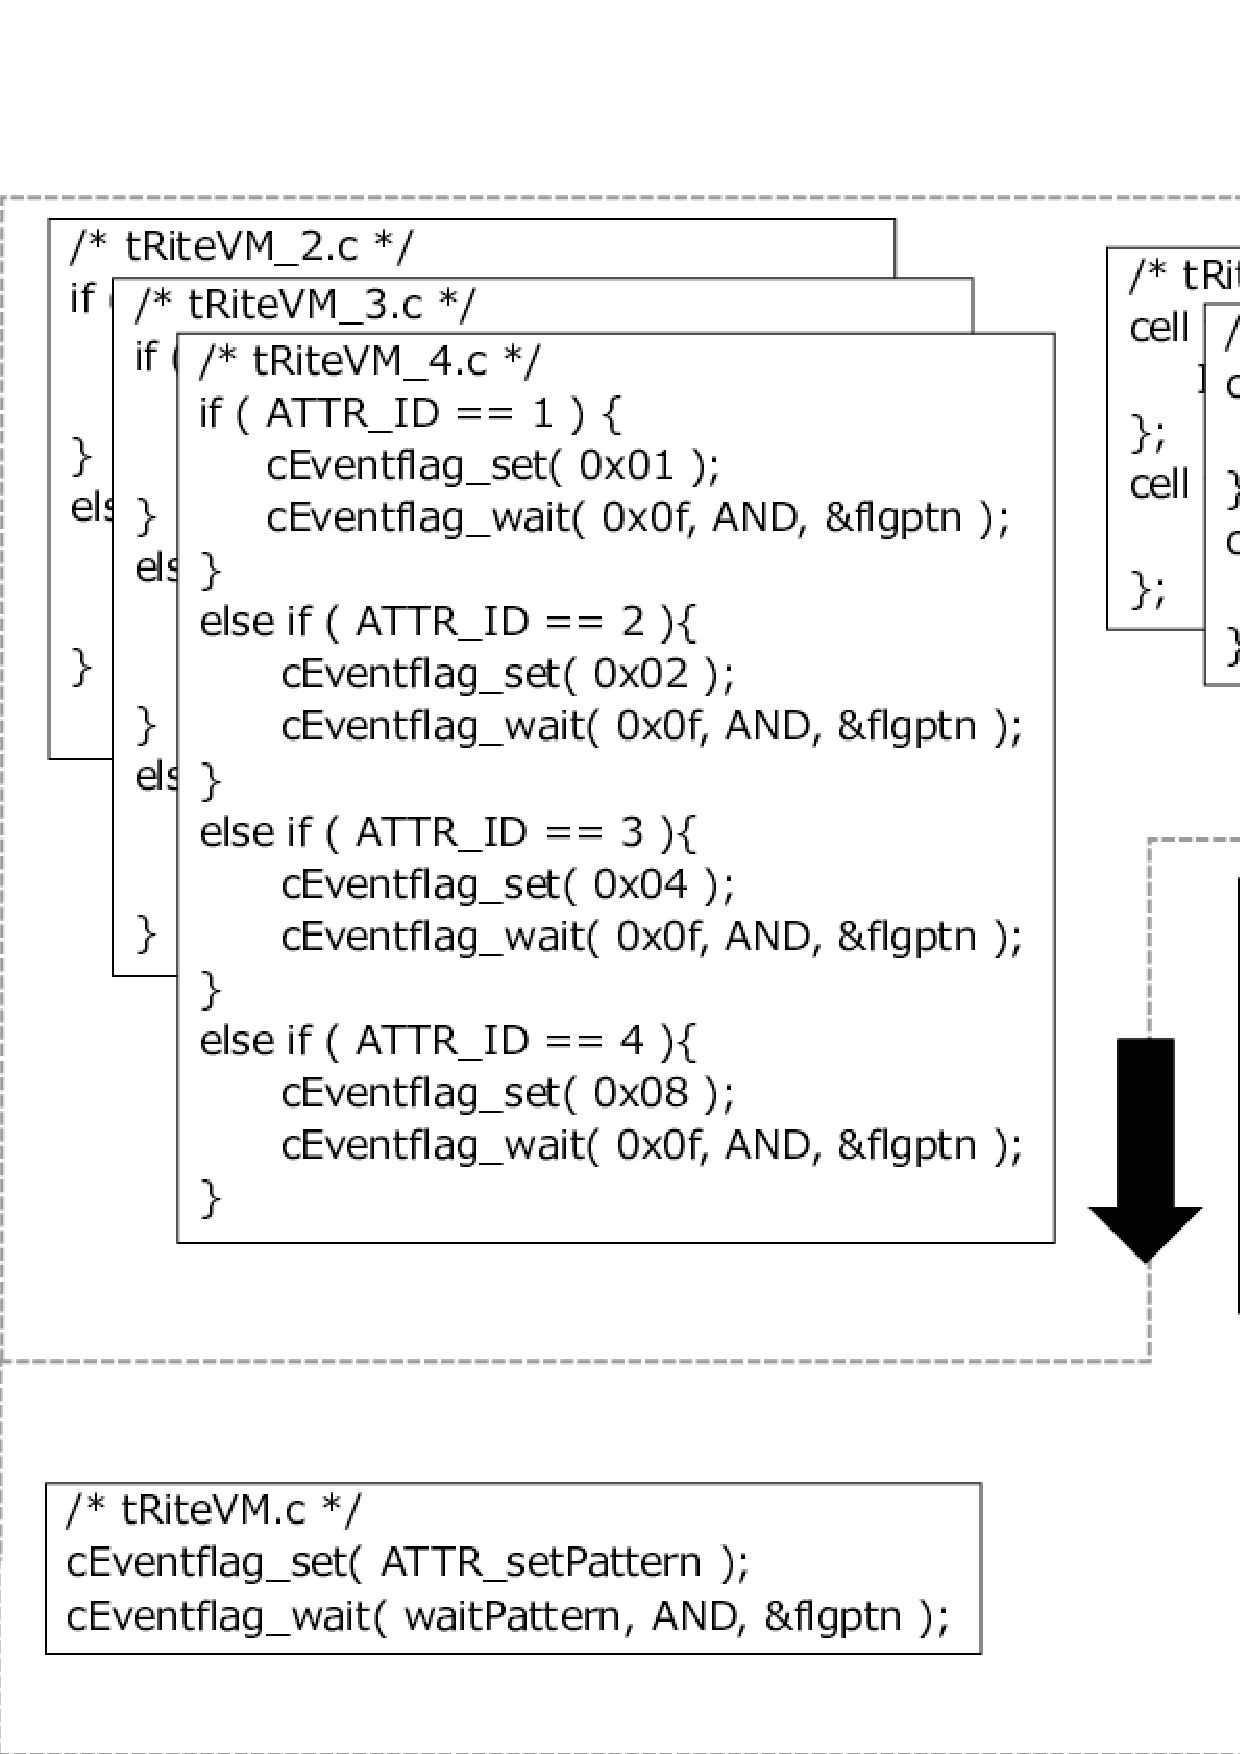
\includegraphics[width=8cm,clip]{../EMSOFT2016/figure/Eventflag.pdf}
    \caption{The design for Eventflag using TECS {\scriptsize *only differences}}
    \label{fig:Eventflag}
\end{figure}
 
\subsection{Benefits of Component-Based Development}
この章では,コンポーネントベース開発の利点を使った設計について述べる.

提案フレームワークでは,RiteVMやRiteVMスケジューラ,イベントフラグはコンポーネントとして提供されているため,開発者はそれらのコンポーネントを容易に付け外し,再利用することができる.
例えば,RiteVMスケジューラの機能を外したい場合,図\ref{celltype_cyclic_handler},\ref{build_cyclic_handler}に示されるcdlファイルを{\it //import($<$tRiteVMScheduler.cdl$>$);}のようにコメントアウトすることで容易に実現できる.
開発者は,カーネルのコンフィグレーションファイルを修正する手間を省くことができる.

それに加えて,コンポーネントベース開発ではコード量を減らすことができる.
提案フレームワークでは,イベントフラグにこの利点は見られる.
図\ref{fig:Eventflag}に示されるように,イベントフラグのセットパターンと待ちパターンを属性として定義する.
{\it cEventflag\_set(ATTR\_setPattern)}に見られるこの設計によって,if文なしでプログラムを記述でき,RiteVMの数に関わらず同じCファイルを使用できる.
さらに,TECSのオプションである{\it [optional]}によって,呼び口が結合した場合のみ処理を行うため,イベントフラグの結合を切った場合にでも同じCファイルを利用することができる.

\section{Experimental Evaluation}
\label{sec:Evaluation}
This section mentions experimental results and their consideration.
To analyze the advantages of the proposed framework, the evaluations are performed as follows.
\begin{itemize}
%    \item Execution time of the platform
    \item Size and time for transferred mruby bytecodes
    \item Execution time with singletasking, co-routine, and multitasking
    \item Overhead for cyclic time
%    \item Synchronization of mruby applications
    \item Code size using the benefit of CBD 
\end{itemize}

These evaluations are performed in order to indicate that an mruby bytecode loader improves the software development efficiency, and that the proposed multitask processing effectively executes compared with singletasking or co-routine, and also the overhead of the cyclic period.
This paper demonstrates the proposed system on a LEGO MINDSTORMS EV3 (300MHz ARM9-based Sitara AM1808 system-on-a-chip) compiled with gcc 4.9.3 -O2 and mruby version 1.2.0.

The size, load process time, and compilation time for mruby application and mruby application including library is shown in Table \ref{tab:size_and_time}.
The overhead of load processing is 50.933 msec, which it takes to load a zero bytes bytecode.
Similarly, the overhead of compilation is 46.9 msec, which it takes to compile a zero bytes program.
The mruby application bytecode is smaler and faster than that of including mruby libraries in all terms.
The difference becomes larger as the number of RiteVMs increases because it takes the 50 msec overhead per one RiteVM. 
%In the proposed framework, developers send only mruby application and prepare mruby library in advance.
%Therefore, the design can send the bytecode faster.
In addition, the design can save the time to connect a storage/ROM device to restart an OS.
These advantages lead improvement of the software development efficiency.

\begin{table}[t]
    \centering
    \caption{Comparison of the size and load process time between an mruby application including mruby libraries and not}
    \begin{tabular}{c||c|c|c}
                            & App\&Lib     & App        &   App\&Lib/App  \\ \hline
          Bytecode Size     & 14,044 bytes & 199 bytes  &   $\times$70.6          \\ %\hline
          Load Process Time & 305.081 msec & 7.774 msec &   $\times$39.2          \\
          Compilation Time  & 8.7 msec     & 0.3 msec   &   $\times$29.0          \\
    \end{tabular}
    \label{tab:size_and_time}
\end{table}

The comparison of the application execution time with singletasking, co-routine, and multitasking is shown in Figure \ref{fig:comparison_s_c_m}.
The 100,000 times loop program is used as mruby application for evaluation of execution time.
In detail, the singletask program loops 100,000 times, and the multitask and co-routine programs loop 50,000 times in each task.
In Figure \ref{fig:comparison_s_c_m}, the cyclic time of the cyclic handler for multitasking is one msec.
While multitask's execution time is slower than singletask's, co-routine takes more time than multitask to execute an mruby application.
This result shows the proposed design is superior to co-routine in terms of execution time.
The overhead of multitask is about 5 \% ($(multitask-singletask)/multitask$).
Switching tasks' overhead is also evaluated, that is about three $\mu$sec on average.
%The number of switching tasks is from 500 to 600 because singletasking process in Figure \ref{fig:comparison_s_c_m} takes about 540 msec.
%Therefore, the overhead of multitasking is 0.5 \% or less, and multitasking can be used without the overhead.
The scheuler interrupts and switches tasks, which causes this overhead.


\begin{figure}[t]
    \centering
    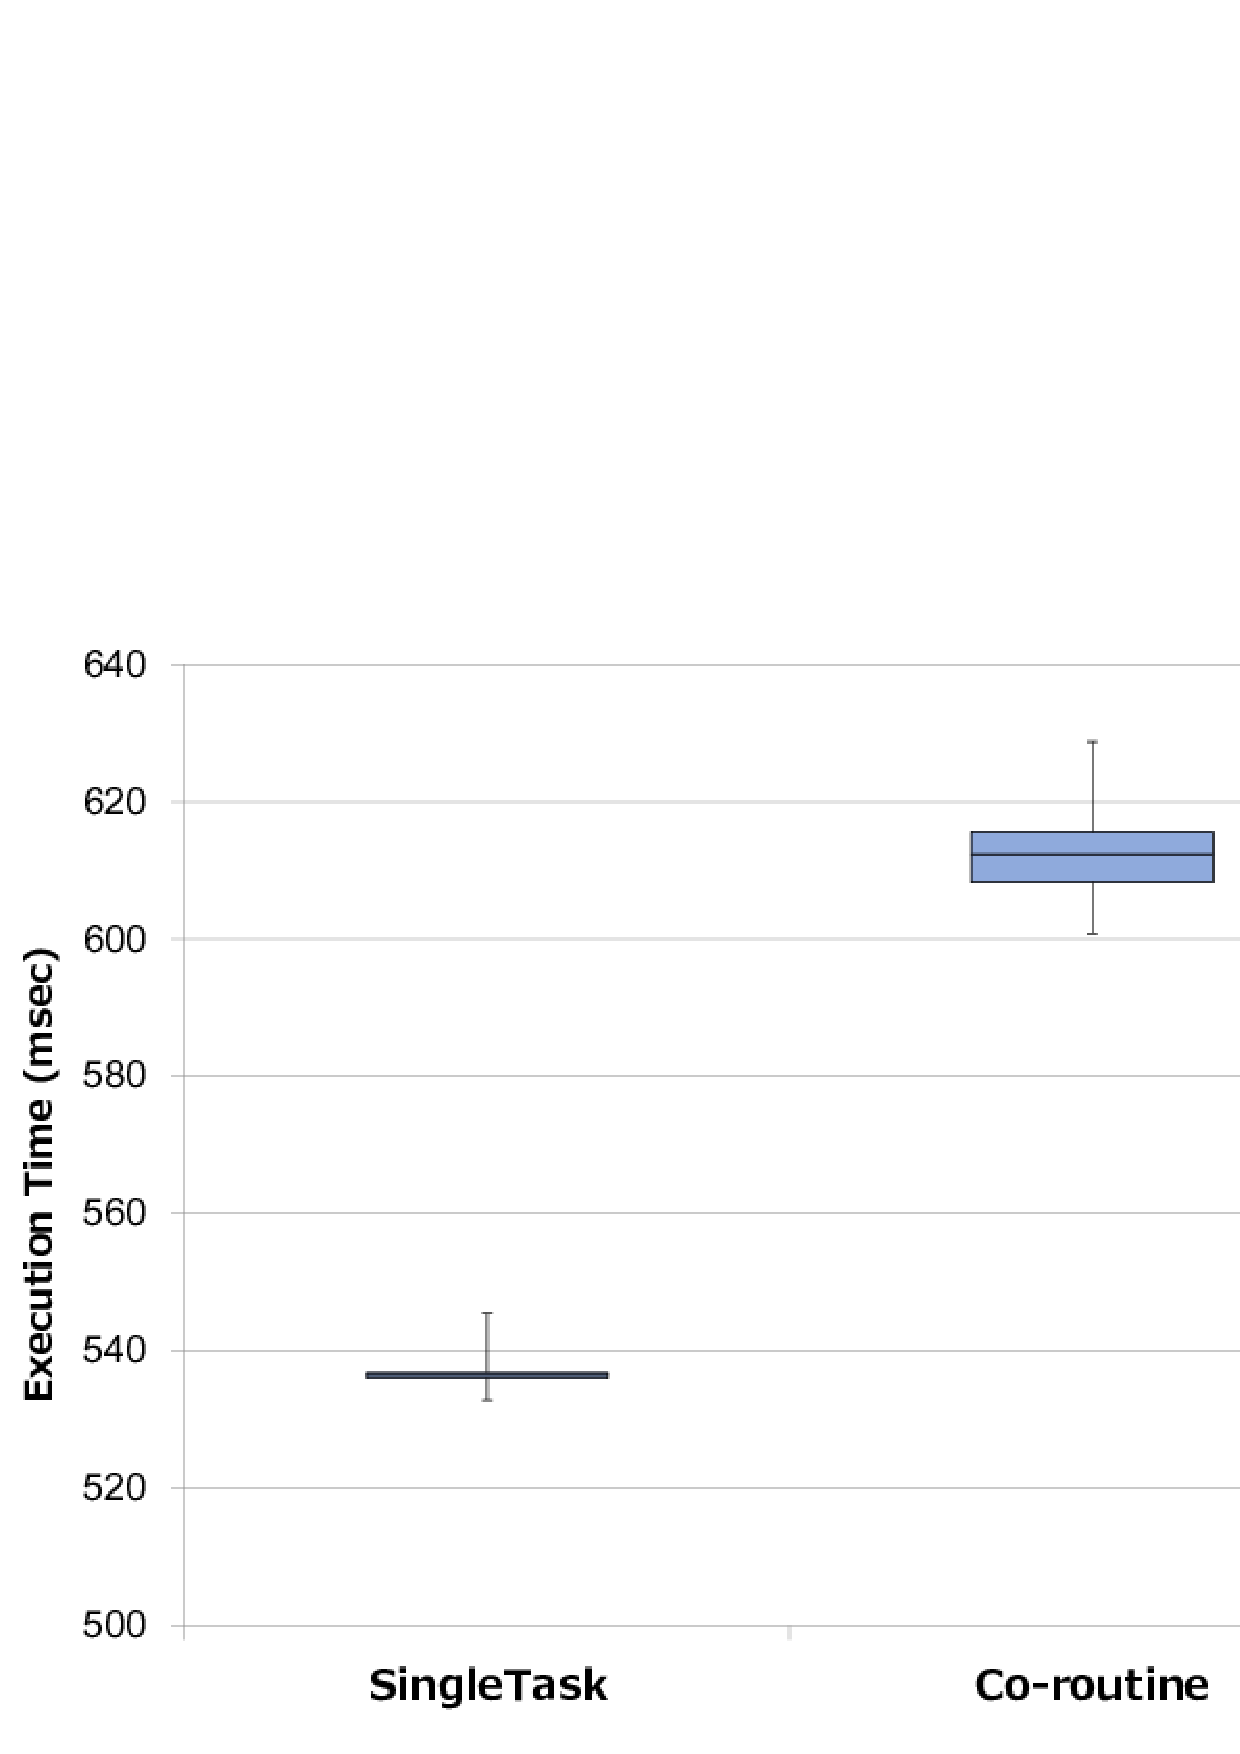
\includegraphics[width=8cm,clip]{../EMSOFT2016/figure/comparison_s_c_m.pdf}
    \caption{Comparison of the application execution time with singletask, co-routine, and multitask}
    \label{fig:comparison_s_c_m}
\end{figure}

Figure \ref{fig:comparison_msec} shows the execution time of multitasking with the cyclic handler.
A lower limit of the cyclic time is one msec due to the specification of TOPPERS/HRP2, the used RTOS.
More than 10 msec do not be evaluated in this paper because it is thought the larger cyclic time influences applications.
Each execution time of cyclic period is the same as the others.
That is because the overhead of switching tasks (about 3 $\mu$sec) is small in comparison with the execution time.
This results also shows the overhead becomes smaller as the cyclic time is larger, because the overhead depends on the number of switching tasks.
The smaller cyclic time is better in multitasking due to concurrent and/or parallel processing.

\begin{figure}[t]
    \centering
    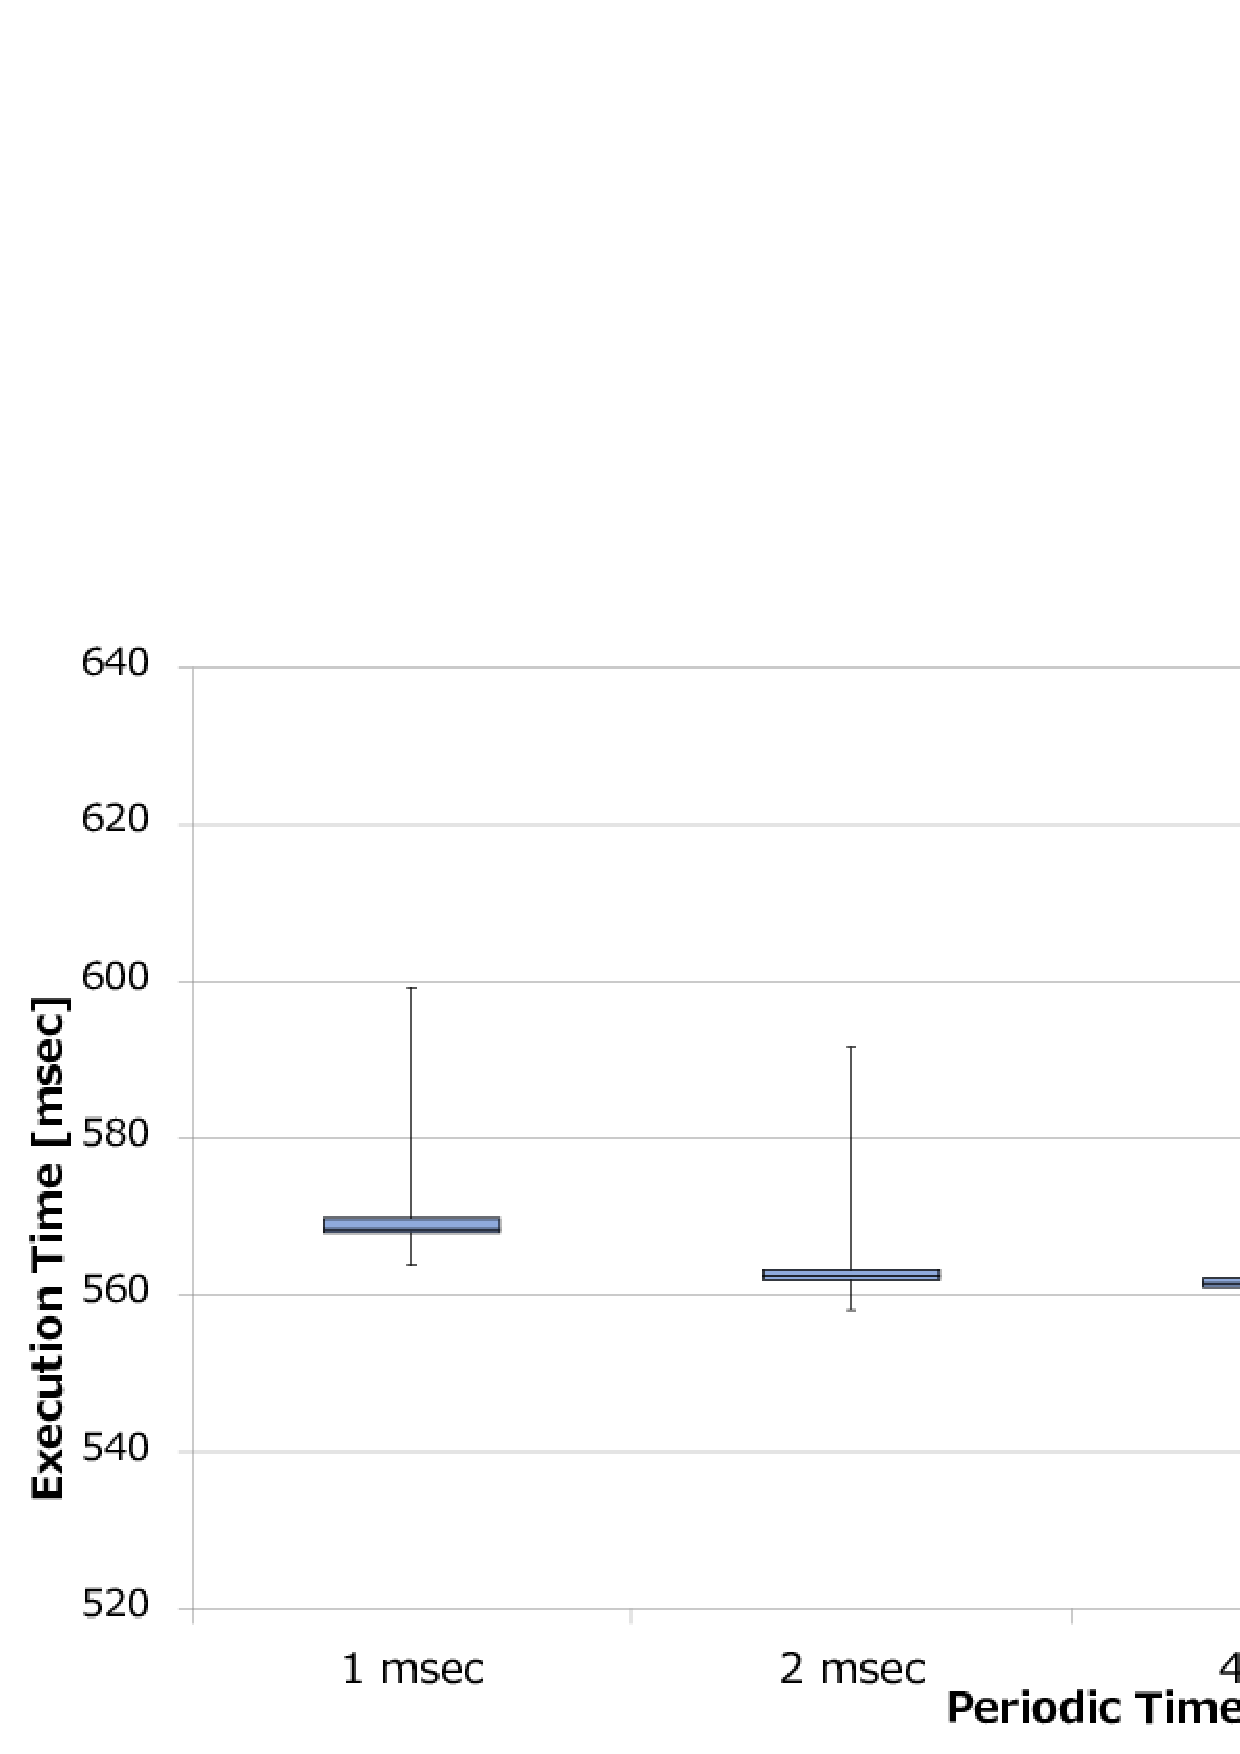
\includegraphics[width=8cm,clip]{../EMSOFT2016/figure/comparison_msec.pdf}
    \caption{Comparison of the overhead for each cyclic period of calling rotateReadyQueue}
    \label{fig:comparison_msec}
\end{figure}

To indicate the superior of component-based development, the comparison of code lines between two .c files is shown in Table \ref{tab:codesize}.
(A) and (B) mean the source files in the upper and lower of Figure \ref{fig:Eventflag}, respectively. 
In terms of .c, (B)'s lines do not increase even if the number of RiteVMs increases, while (A)'s lines increase in proportion to the number.
(B) is not modified, and can be utilized regardless of the number of RiteVMs.
Moreover, lines of two .cdl files are equal.
The skillfull component-based development brings this advantage such as the decrease of code lines, which leads high productivity and high maintainability.

\begin{table}[t]
    \centering
    \caption{Lines of .c and .cdl file for the number of RiteVM}
    \begin{tabular}{c||cc|c}
                & (A)       & (B)     & Diff  \\ \hline
        .c      & 134$+$8$\times$$\alpha $  & 130     & 4$+$8$\times$$\alpha$ \\
        .cdl    & 25$+$18$\times$$\alpha$   & 25$+$18$\times$$\alpha$ & 0     \\
        \multicolumn{3}{l}{  }\\
        \multicolumn{3}{l}{{\small $\alpha$} : {\scriptsize the number of RiteVM}}
    \end{tabular}
    \label{tab:codesize}
\end{table}

\section{Related Work}
\label{sec:Related work}

\begin{table*}[t]
    \centering
    \caption{Comparion of the proposed and previous work}
    \begin{tabular}{c||c|ccccccc}
        & Bluetooth Loader & \shortstack{Call\\C Function} & \shortstack{Legacy Code of\\Embedded System} & \shortstack{VM\\Managenment} & \shortstack{VM\\Scheduler} & \shortstack{Synchronization of\\Application} & Co-routine \\ \hline
        python-on-a-chip \cite{url:python-on-a-chip} &            &            &            &            &             &            & \checkmark \\
        Owl system \cite{par:owl}                    &            & \checkmark & Partially  &            &             &            & \checkmark \\
        eLua \cite{url:eLua}                         &            & \checkmark & Partially  &            &             &            & \checkmark \\
        mruby \cite{par:mruby}                       &            & \checkmark &            &            &             &            & \checkmark \\
        mruby on TECS \cite{par:mrubyonTECS}         &            & \checkmark & \checkmark & \checkmark &             &            & \checkmark \\
        Proposed framework                           & \checkmark & \checkmark & \checkmark & \checkmark & \checkmark  & \checkmark & \checkmark \\
    \end{tabular}
    \label{tab:comparison}
\end{table*}
The open-source run-time systems for scripting languages have been proposed such as follow:
python-on-a-chip \cite{url:python-on-a-chip}, the Owl system \cite{par:owl}, eLua \cite{url:eLua}, mruby \cite{par:mruby}, \cite{url:mruby}, and mruby on TECS \cite{par:mrubyonTECS}.

python-on-a-chip (p14p) is a Python run-time system that uses a reduced Python VM called PyMite.
The VM runs a significant subset of Python language with few resources on a microcontroller.
p14p can run multiple stackless green threads.

The Owl system is an embedded Python run-time system.
The Owl is a complete system for ARM Cortex-M3 microcontrollers.
The Owl toolchain produces relocatable memory images, that are directly runnable on the microcontroller, from Python code objects.
The interpreter of the Owl system is the same as that of python-on-a-chip.

eLua offers the full implementation of Lua programming language to the embedded systems.
Lua is one of the most popular script languages for embedded systems \cite{url:Lua}, \cite{par:Lua}.
Lua supports co-routine, referred to collaborative multitasking.
A co-routine in Lua is used as an independently executed thread.
A co-routine can just suspend and resume multiple routines.
Thus, a Lua co-routine is not like multitasks in multitask systems.

mruby, the lightweight implementation of the Ruby language, has been proposed for embedded systems.
mruby programs can run on a RiteVM, which is the VM for mruby and reads the mruby bytecode.
mruby has supported co-routine, but not supported multitasking for RTOSs.

mruby on TECS is a component-based framework for running mruby programs.
The programs on mruby on TECS can execute about 100 times faster than the mruby programs.
Software can be also developed with component base by mruby on TECS.
Although multitasking has been supported in the current mruby on TECS, developers need to be familiar with functions of an RTOS to use multitasking.
The co-routine is supported as same as mruby.

Table \ref{tab:comparison} shows a comparison between the proposed framework and previous work.
The proposed framework supports the loader, the VM scheuler, and synchronization of application.
 
\section{Conclusion}
\label{sec:Conclusion}
This paper has presented an extended framework of mruby on TECS: mruby bytecode loader using Bluetooth and RiteVM scheuler.
The loader provides developers with the software development efficiency without rewriting a storage/ROM device and restarting an OS.
The proposed framework can be applied to many kinds of embedded systems  because the loader can use not only Bluetooth also wired serial connection.
%Thus, the proposed framework can be utilized on the deveces without Bluetooth.
The RiteVM scheuler makes multitasking more easily than the current mruby on TECS.
In the evaluation, experimental results of the loader and the RiteVM scheduler show their advantages.
The loader can improve the software development efficiency on mruby on TECS.
The RiteVM sceduler has the effectiveness in terms of execution time and ease of use compared with singletasking and co-routine.
%because of the low overhead.

The proposed framework is developed in component-base by TECS.
The facilities such as RiteVMs, the RiteVM scheuler, and Eventflag are implemented as components.
Therefore, developers can easily add or remove the functionalities as necessary, and also reuse them.
Developers can choose fair scheduling or fixed-priority scheduling since the RiteVM scheuler can be easily removed.
Component-based development can increase productivity and decrease complexity.

In the future, the mruby bytecode loader using Bluetooth will be supported to handle multiple bytecodes and run the application in multi-VM.
Moreover, the .cdl files for RiteVM and mruby-TECS bridge are generated automatically using a plugin, and developers can send a bytecode with ZMODEM protocol on the command line.


%%%%%%%%%%%% Reference %%%%%%%%%%%%%%%%%%%%%%%%%%%%%%%%%%%%%%%%%%%%%%
\bibliographystyle{ipsj_v2/UTF8/ipsjunsrt-e}
\bibliography{../EMSOFT2016/ref}

\begin{biography}
\profile{m,E}{情報 太郎}{1970年生.1992年情報処理大学理学部情報科学科卒業.
1994年同大学大学院修士課程修了.同年情報処理学会入社.オンライン出版の研究
に従事.電子情報通信学会,IEEE,ACM 各会員.}
%
\profile{n}{処理 花子}{1960年生.1982年情報処理大学理学部情報科学科卒業.
1984年同大学大学院修士課程修了.1987年同博士課程修了.理学博士.1987年情報処
理大学助手.1992年架空大学助教授.1997年同大教授.オンライン出版の研究
に従事.2010年情報処理記念賞受賞.電子情報通信学会,IEEE,IEEE-CS,ACM
各会員.}
%
\profile{h,L}{学会 次郎}{1950年生.1974年架空大学大学院修士課程修了.
1987年同博士課程修了.工学博士.1977年架空大学助手.1992年情報処理大学助
教授.1987年同大教授.2000年から情報処理学会顧問.オンライン出版の研究
に従事.2010年情報処理記念賞受賞.情報処理学会理事.電子情報通信学会,
IEEE,IEEE-CS,ACM 各会員.}
\end{biography}

\end{document}
